\documentclass[main.tex]{subfiles}
\begin{document}

\chapter{Re\"ele en complexe getallen}
\label{cha:reele-en-complexe-getallen}

\section{De rationale getallen en hun structuur}
\label{sec:de-rati-getall}

\begin{de}
  De \term{gehele getallen}, genoteerd als $\mathbb{Z}$.
  \[ \mathbb{Z} = \mathbb{N} \cup \{ -n \mid n\in \mathbb{N} \}  \]
\end{de}

\begin{de}
  De \term{rationale getallen}, genoteerd als $\mathbb{Q}$.
  \[ \mathbb{Q} = \{ \nicefrac{n}{m} \mid n\in \mathbb{Z}, m\in \mathbb{Z}, m \neq 0 \} \]
\end{de}


\begin{de}
  Een \term{veld} $\mathbb{F},+,\cdot$ is een verzameling $\mathbb{F}$ met twee bewerkingen $+$ en $\cdot$ met de volgende eigenschappen.
  \begin{itemize}
  \item $+$ is associatief:
    \[ \forall f,g,h \in \mathbb{F}:\ (f+g)+h = f+(g+h) \]
  \item Er bestaat een (uniek) neutraal element $0$ voor $+$:
    \[ \forall f\in \mathbb{F}:\ f + 0 = f = 0 + f \]
  \item Elk element $x$ heeft een (uniek) invers element $-x$ voor $+$:
    \[ \forall f\in \mathbb{F}: \exists (-f) \in \mathbb{F}: \ f + (-f) = 0 = (-f) + f \]
  \item $+$ is commutatief:
    \[ \forall f,g \in \mathbb{F}:\ f+g = g+f \]
  \item $\cdot$ is associatief:
    \[ \forall f,g,h \in \mathbb{F}:\ (f\cdot g) \cdot h = f\cdot (g\cdot h) \]
  \item Er bestaat een (uniek) neutraal element $1$ voor $\cdot$:
    \[ \forall f\in \mathbb{F}:\ f \cdot 1 = f = 1 \cdot f \]
  \item Elk element $x$ heeft een (uniek) invers element $x^{-1}$ voor $\cdot$:
    \[ \forall f\in \mathbb{F}: \exists f^{-1} \in \mathbb{F}: \ f \cdot f^{-1} = 0 = f^{-1} \cdot f \]
  \item $\cdot$ is commutatief:
    \[ \forall f,g \in \mathbb{F}:\ f\cdot g = g \cdot f \]
  \item $\cdot$ is distributief ten opzichte van $+$:
    \[ \forall f,g,h \in \mathbb{F}:\ f \cdot (g+h) = (f \cdot g) + (f \cdot h) \]
  \end{itemize}
\end{de}

\begin{de}
  \label{de:totaal-geordend-veld}
  Zij $\mathbb{F},+,\cdot$ een veld met een totale orderelatie $\le$, dan noemen we het een \term{totaal geordend veld} als aan de volgende eigenschappen voldaan is.
  \begin{itemize}
  \item $\forall x,y,z \in \mathbb{F}:\ x \le y \Rightarrow (x+z) \le (y+z)$
  \item $\forall x,y,z \in \mathbb{F}:\ x \le y \wedge 0 \le z \Rightarrow x\cdot z \le y\cdot z$
  \end{itemize}
\end{de}

\begin{pr}
  $\mathbb{Q}$ is een totaal geordend veld.

  \begin{proof}
    We bewijzen elk deel appart.
    \begin{itemize}
    \item $\mathbb{Q}$ is een veld.
      \begin{itemize}
      \item $+$ is associatief:
        \[ 
        \begin{array}{rrl}
          \forall \frac{f_{t}}{f_{n}},\frac{g_{t}}{g_{n}},\frac{h_{t}}{h_{n}} \in \mathbb{Q}:\
          &\left(\frac{f_{t}}{f_{n}} + \frac{g_{t}}{g_{n}}\right) + \frac{h_{t}}{h_{n}}
          &= \frac{f_{t}g_{n} + g_{t}f_{n}}{f_{n}g_{n}} + \frac{h_{t}}{h_{n}}\\
          &&= \frac{f_{t}g_{n}h_{n} + g_{t}f_{n}h_{n} + h_{t}f_{n}g_{n}}{f_{n}g_{n}h_{n}}\\
          &&=  \frac{f_{t}}{f_{n}} + \frac{g_{t}h_{n} + h_{t}g_{n}}{g_{n}h_{n}}\\
          &&= \frac{f_{t}}{f_{n}} + \left(\frac{g_{t}}{g_{n}} + \frac{h_{t}}{h_{n}}\right)\\
        \end{array}
        \]
        We gebruiken hier dat $+$ en $\cdot$ associatief en commutatief zijn in $\mathbb{Z}$
      \item Er bestaat een (uniek) neutraal element $0$ voor $+$:
        \[
        \begin{array}{rrl}
          \forall \frac{f_{t}}{f_{n}}\in \mathbb{Q}:\
          &\frac{f_{t}}{f_{n}} + \frac{0}{1}
          &= \frac{f_{t} + 0}{1}\\
          &&= \frac{f_{t}}{f_{n}}\\
          &&= \frac{0 + f_{t}}{1}\\
          &&= 0 +  \frac{f_{t}}{f_{n}}\\
        \end{array}
        \]
        We gebruiken hier dat $0$ het neutraal element is voor $+$ in $\mathbb{Z}$.
      \item Elk element $x$ heeft een (uniek) invers element $-x$ voor $+$:
        \[
        \begin{array}{rrl}
          \forall \frac{f_{t}}{f_{n}}\in \mathbb{Q}: \exists (-f) = \frac{-f_{t}}{f_{n}} \in \mathbb{F}: \ 
          &\frac{f_{t}}{f_{n}} + \frac{-f_{t}}{f_{n}}
          &= \frac{f_{t}f_{n} + (-f_{t}f_{n})}{f_{n}^{2}}\\
          &&= \frac{0}{f_{n}^{2}}\\
          &&= 0 \\
          &&= \frac{0}{f_{n}^{2}}\\
          &&= \frac{-f_{t}f_{n} + f_{t}f_{n}}{f_{n}^{2}}\\
          &&= \frac{-f_{t}}{f_{n}} + \frac{f_{t}}{f_{n}}\\
        \end{array}
        \]
        We gebruiken hier dat $-x$ het invers element is van $x$ voor $+$ in $\mathbb{Z}$. 
      \item $+$ is commutatief:
        \[
        \forall \frac{f_{t}}{f_{n}},\frac{g_{t}}{g_{n}} \in \mathbb{Q}:\
        \frac{f_{t}}{f_{n}} + \frac{g_{t}}{g_{n}}
        = \frac{f_{t}g_{n}+g_{t}f_{n}}{f_{n}g_{n}}\\ 
        = \frac{g_{t}}{g_{n}} + \frac{f_{t}}{f_{n}}\\
        \]
        We gebruiken hier dat $\cdot$ commutatief is en $+$ associatief in $\mathbb{Z}$.
      \item $\cdot$ is associatief:
        \[
        \forall \frac{f_{t}}{f_{n}},\frac{g_{t}}{g_{n}},\frac{h_{t}}{h_{n}} \in \mathbb{Q}:\
        \left(\frac{f_{t}}{f_{n}} \cdot \frac{g_{t}}{g_{n}}\right) \cdot \frac{h_{t}}{h_{n}}
        =\frac{f_{t}g_{t}}{f_{n}g_{n}} \cdot \frac{h_{t}}{h_{n}}
        =\frac{f_{t}g_{t}h_{t}}{f_{n}g_{n}h_{n}}
        =\frac{f_{t}}{f_{n}} \cdot \frac{g_{t}h_{t}}{g_{n}h_{n}}
        \]
        We gebruiken hier dat $\cdot$ commutatief is in $\mathbb{Z}$.
      \item Er bestaat een (uniek) neutraal element $1$ voor $\cdot$:
        \[
        \begin{array}{rrl}
          \forall \frac{f_{t}}{f_{n}}\in \mathbb{Q}:\
          &\frac{f_{t}}{f_{n}} \cdot \frac{1}{1}
          &= \frac{f_{t}\cdot 1}{1 \cdot 1}\\
          &&= \frac{f_{t}}{f_{n}}\\
          &&= \frac{1\cdot f_{t}}{1 \cdot 1}\\
          &&= 1 \cdot \frac{f_{t}}{f_{n}}\\
        \end{array}
        \]
        We gebruiken hier dat $1$ het neutraal element is voor $\cdot$ in $\mathbb{Z}$.
      \item Elk element $x$ heeft een (uniek) invers element $x^{-1}$ voor $\cdot$:
        \[
        \forall \frac{f_{t}}{f_{n}}\in \mathbb{Q}: \exists \frac{f_{t}}{f_{n}}^{-1} = \frac{f_{n}}{f_{t}} \in \mathbb{F}: \
        = \frac{f_{t}}{f_{n}}\frac{f_{n}}{f_{t}}
        = \frac{f_{t}f_{n}}{f_{t}f_{n}}
        = 1
        = \frac{f_{n}f_{t}}{f_{t}f_{n}}
        = \frac{f_{n}}{f_{t}}\frac{f_{t}}{f_{n}}
        \]
        We gebruiken hier dat $\cdot$ commutatief is in $\mathbb{Z}$.
      \item $\cdot$ is commutatief:
        \[
        \forall \frac{f_{t}}{f_{n}},\frac{g_{t}}{g_{n}} \in \mathbb{Q}:\
        \frac{f_{t}}{f_{n}} \cdot \frac{g_{t}}{g_{n}}
        = \frac{f_{t}g_{t}}{f_{n}g_{n}}
        = \frac{g_{t}}{g_{n}} \cdot \frac{f_{t}}{f_{n}}
        \]
        We gebruiken hier dat $\cdot$ commutatief is in $\mathbb{Z}$.
      \item $\cdot$ is distributief ten opzichte van $+$:
        \[
        \begin{array}{rrl}
          \forall \frac{f_{t}}{f_{n}},\frac{g_{t}}{g_{n}},\frac{h_{t}}{h_{n}} \in \mathbb{Q}:\ 
          &\frac{f_{t}}{f_{n}} \cdot \left(\frac{g_{t}}{g_{n}} + \frac{h_{t}}{h_{n}} \right)
          &= \frac{f_{t}}{f_{n}} \cdot \frac{g_{t}h_{n}+h_{t}g_{n}}{g_{n}h_{n}}\\
          &&= \frac{f_{t}\cdot (g_{t}h_{n}+h_{t}g_{n})}{f_{n}g_{n}h_{n}}\\
          &&= \frac{(f_{t} \cdot g_{t}h_{n}) + (f_{t}\cdot h_{t}g_{n})}{f_{n}g_{n}h_{n}}\\
          &&= \frac{f_{t}g_{t}}{f_{n}g_{n}} + \frac{f_{t}h_{t}}{f_{n}h_{n}}\\
        \end{array}
        \]
      \end{itemize}
    \item $\mathbb{Q}$ is totaal geordend veld.
      \begin{itemize}
      \item
        \[
        \forall \frac{f_{t}}{f_{n}},\frac{g_{t}}{g_{n}},\frac{h_{t}}{h_{n}} \in \mathbb{Q}:\ 
        \frac{f_{t}}{f_{n}} \le \frac{g_{t}}{g_{n}}
        \Rightarrow
        \frac{f_{t}}{f_{n}}+\frac{h_{t}}{h_{n}} \le \frac{g_{t}}{g_{n}}+\frac{h_{t}}{h_{n}}
        \]
        \extra{vanuit welke axioma's bewijzen we dit?}
      \item $\forall x,y,z \in \mathbb{F}:\ x \le y \wedge 0 \le z \Rightarrow x\cdot z \le y\cdot z$
        \extra{vanuit welke axioma's bewijzen we dit?}
      \end{itemize}
    \end{itemize}
  \end{proof}
\end{pr}

\begin{pr}
  \label{pr:geordend-veld-optelling-ongelijkheden}
  Zij $\mathbb{F},+,\cdot,\le$ een totaal geordend veld.
  \[ \forall a,b,c,d \in \mathbb{F}:\ a\le b \wedge c \le d \Rightarrow (a+c) \le (b+d) \]

  \begin{proof}
    We gebruiken enkel de eerste eigenschap in de definitie van een totaal geordend veld.
    Omdat $a\le b$ geldt geldt ook $a + c \le b+c$.
    Bovendien geldt $c+b \le d+b$ omdat $c\le d$ geldt.
    Omdat $+$ commutatief is in $\mathbb{F}$, geldt dan ook het volgende:
    \[ a+c \le b+c \le b+d\]
  \end{proof}
\end{pr}

\begin{pr}
  \label{pr:geordend-veld-ongelijkheid-maal-min-een}
  Zij $\mathbb{F},+,\cdot,\le$ een totaal geordend veld.
  \[ \forall a,b\in \mathbb{F}:\ a \le b \Rightarrow -b \le -a \]

  \begin{proof}
    Bewijs uit het ongerijmbde\\
    Stel $a \le b$ en $-b > -a$ (dus $-a \le b$).
    Omdat $\mathbb{F}$ een totaal geordend veld is, volgt uit $-a \le -b$ zowel $a \le -b+2a$ en $-a+2b \le -b$.
    Tel deze ongelijkheden op\prref{pr:geordend-veld-optelling-ongelijkheden} om $2b \le 2a$ te bekomen.
    Uit $a\le b$ volgt echter dat $2a \le 2b$ geldt (tel immers $a\le b$ bij zichzelf op).
    Contradictie.
  \end{proof}
\end{pr}

\begin{pr}
  \label{pr:geordend-veld-tegengestelde-wisselt-teken}
  Zij $\mathbb{F},+,\cdot,\le$ een totaal geordend veld.
  \[ \forall b \in \mathbb{F}:\ 0 \le b \Leftrightarrow -a \le 0 \]

  \begin{proof}
    Gebruik in propositie \ref{pr:geordend-veld-ongelijkheid-maal-min-een} $a=0$.
  \end{proof}
\end{pr}

\begin{pr}
  \label{pr:geordend-veld-ongelijkheid-vermenigvuldiging}
  Zij $\mathbb{F},+,\cdot,\le$ een totaal geordend veld.
  \[ \forall a,b \in \mathbb{F}:\ 0 \le a \wedge 0 \le b \Rightarrow 0 \le ab \]

  \begin{proof}
    Omdat $\mathbb{F}$ een geordend veld is, volgt uit $0\le a$ dat $0b \le ab$ geldt vanwege $0 \le b$.
    Omdat $0$ het nulelement is van $\mathbb{F}$ geldt $0b = 0$.
  \end{proof}
\end{pr}

\begin{pr}
  \label{pr:nul-kleiner-dan-een}
  Zij $\mathbb{F},+,\cdot,\le$ een totaal geordend veld.
  \[ 0 < 1 \]

  \begin{proof}
    Bewijs uit het ongerijmde\\
    Stel dat $1 \le 0$ geldt, dan moet $1<0$ gelden omdat in een veld $1$ verschilt van $0$.
    Tel hierbij $-1$ op, dan bekomen we $0 \le -1$.
    Vanwege de tweede definierende eigenschap van een totaal geordend veld moet dan uit $1 \le 0$ ook $-1 \le 0$ volgen, maar dat is in strijd met $0 \le -1$ omdat $0$ verschilt van $1$.
  \end{proof}
\end{pr}

\begin{pr}
  \label{pr:geordend-veld-inverse-zelfde-teken}
  Zij $\mathbb{F},+,\cdot,\le$ een totaal geordend veld.
  \[ \forall a \in \mathbb{F}_{0}:\ 0 \le a \Rightarrow 0 \le a^{-1}\]

  \begin{proof}
    Bewijs uit het ongerijmde:
    Stel $0 \le a$ maar ook $a^{-1} < 0$ geldt.
    We mogen die tweede ongelijkheid dan vermenigvuldigen met $a$ om $aa^{-1}< 0$ te bekomen.
    Dit zou $1<0$ betekenen en dat is in contradictie met propositie \ref{pr:nul-kleiner-dan-een}.
  \end{proof}
\end{pr}

\begin{pr}
  \label{pr:geordend-veld-inverse-ongelijkheid-rekenregel}
  Zij $\mathbb{F},+,\cdot,\le$ een totaal geordend veld.
  \[ \forall a,b \in \mathbb{F}_{0}^{+}:\  a \le b \Rightarrow b^{-1} \le a^{-1}\]

  \begin{proof}
    Omdat zowel $0 \le a$ en $0 \le b$ geld, mogen we $a\le b$ vermenigvuldigen met $a^{-1}$ en $b^{-1}$\prref{pr:geordend-veld-inverse-zelfde-teken} om $b^{-1} \le a^{-1}$ te bekomen.
  \end{proof}
\end{pr}

\begin{st}
  $\sqrt{2}$ is geen element van $\mathbb{Q}$.
  \extra{bewijs}
\end{st}

\begin{st}
  $\mathbb{Q}$ heeft de supremumeigenschap niet.
\end{st}

\begin{st}
  De stelling van rolle geldt niet in $\mathbb{Q}$.
  \extra{verwijzen naar een plaats met betere uitleg.}
\end{st}

\extra{nog een gebrek van $\mathbb{Q}$.}

\subsection{Axiomatische beschrijving van $\mathbb{R}$}
\label{sec:axiom-beschr-van}

\begin{st}
  \label{st:supremumeigenschap-R}
  De \term{supremumeigenschap}\\
  In $\mathbb{R}$ heeft elke niet-lege, naar boven begrensde deelverzameling een supremum.
  \extra{bewijs verder rigoreuzer}
\end{st}

\begin{st}
  Er bestaat, op isomorfisme na, maar \'e\'en totaal geordend veld met de supremumeigenschap.
  \extra{bewijs later}
\end{st}

\begin{pr}
  Er bestaat een unieke afbeelding $i:\ \mathbb{Q} \rightarrow \mathbb{R}$ met de volgende eigenschappen.
  \begin{itemize}
  \item $i(0_{\mathbb{Q}}) = 0_{\mathbb{R}}$
  \item $i(1_{\mathbb{Q}}) = 1_{\mathbb{R}}$
  \item $\forall p,q \in \mathbb{Q}: i(p+_{\mathbb{Q}}q) = i(p) +_{\mathbb{R}} i(q)$
  \item $\forall p,q \in \mathbb{Q}: i(p\cdot_{\mathbb{Q}} q) = i(p) \cdot_{\mathbb{R}} i(q)$
  \item $\forall p,q \in \mathbb{Q}: p \le_{\mathbb{Q}} q \Rightarrow i(p) \le_{\mathbb{R}} i(q)$
  \end{itemize}
  Bovendien is deze afbeelding injectief.

  \begin{proof}
    \begin{itemize}
    \item Uniciteit\\
      We bewijzen dat er slechts \'e\'en $i$ kan bestaan, eerst over $\mathbb{N}$, dan over $\mathbb{Z}$ en tenslotte over $\mathbb{Q}$.
      \begin{itemize}
      \item Beschouw een $n\in \mathbb{N}$.
        Er zijn dan twee gevallen:
        \begin{itemize}
        \item $n = 0_{\mathbb{O}}$:
          Dan moet $i(n)$ $0_{\mathbb{R}}$ zijn vanwege de eerste eigenschap.
        \item $n \neq 0$:
          $n$ is dan als de som van $n$ $1_{\mathbb{Q}}$-tjes te schrijven:\needed
          \[ n = n 1_{\mathbb{Q}} \]
          Vanwege de derde eigenschap is $i(n)$ dan de som van $n$ $1_{\mathbb{R}}$-jes te schrijven.
        \end{itemize}
        Hierdoor ligt $i$ al vast op $\mathbb{N}$. \waarom
      \item Beschouw vervolgens een getal $z\in \mathbb{Z}\setminus \mathbb{N}$.
        Er bestaat dan een getal $n \in \mathbb{N}$ zodat $z$ het tegengestelde is van $n$: $z = -n$.\needed
        De vierde eigenschap zegt ons dan het volgende:
        \[ i(-n) = -i(n) \]
        Hierdoor ligt $i$ al vast op $\mathbb{Z}$. \waarom
      \item Beschouw tenslotte een $q\in \mathbb{Q}$, dan valt $q$ te schrijven als $\nicefrac{n}{m}$ met $n\in \mathbb{Z}$ en $m\in \mathbb{N}_{0}$.
        Uit de derde eigenschap volgt dan dat het volgende moet gelden:
        \[ i(q) = i(n)i(m)^{-1} \]
        Dit vervolledigt de uniciteit van $i$.
      \end{itemize}
    \item Bestaan\\
      Verdergaand op het bewijs van de uniciteit construeren we $i$ achtereenvolgens op $\mathbb{N}$, dan op $\mathbb{Z}$ en dan op $\mathbb{Q}$.
      \extra{bewijzen dat $i$ door $+$ en $\cdot$ gaat}
      \extra{bewijzen dat $i$ goed gedefinieerd is voor $\mathbb{Q}$ (onafhankelijk van de gekozen $m$ en $n$).}
      \extra{bewijzen dat $i$ injectief en stijgend is}
    \end{itemize}
  \end{proof}
\end{pr}

\begin{opm}
  Onder dit morfisme beschouwen we $\mathbb{Q}$ als een deelverzameling van $\mathbb{R}$.
\end{opm}


\begin{lem}
  \label{lem:lemma-van-archimedes}
  Het \term{lemma van Archimedes}\\
  Voor elke $x\in \mathbb{R}$ bestaat er een $n\in \mathbb{N}$ zodat $x < n$ geldt.

  \begin{proof}
    Bewijs uit het ongerijmde\\
    Stel dat er een $x\in \mathbb{R}$ zou bestaan zodat $\forall n \in \mathbb{N}:\ x \ge n$ geldt, dan zou $\mathbb{N}$ naar boven begrensd zijn door die $x$.
    Noem $s$ dan het supremum van $\mathbb{N}$, dat bestaat immers zeker.\needed
    Omdat $s$ de kleinste bovengrens is van $\mathbb{N}$ is $s-1$ zeker geen bovengrens.
    We kunnen dus een $k\in \mathbb{N}$ vinden zodat $s-1$ kleiner is dan $k$.
    $s$ is dan echter kleiner dan $k+1$ en dus geen bovengrens.
  \end{proof}
\end{lem}

\begin{gev}
  $\forall a \in \mathbb{R}_{0}^{+},\ \forall b\in \mathbb{R}:\ \exists n\in N:\ na > b$

  \begin{proof}
    Als $b$ kleiner is dan $a$ is de stelling evident met $n=1$.
    Als $b$ groter is dan of gelijk aan $a$, ga dan als volgt te werk:
    $a^{-1}$ is positief (want $a$ is positief)\prref{pr:geordend-veld-inverse-zelfde-teken}, uit $a \le b$ volgt dus $1 \le \frac{b}{a}$.
    Kies dan een $n\in \mathbb{N}$ groter dan $\frac{b}{a}$, dit kan immers altijd.\lemref{lem:lemma-van-archimedes}
    Vermenigvuldig tenslotte $\frac{b}{a} < n$ met $a$ om de stelling te bekomen.\deref{de:geordend-veld}
  \end{proof}
\end{gev}

\begin{gev}
  \label{gev:er-bestaat-alijd-iets-rationaal-kleiner}
  $\forall \epsilon \in \mathbb{R}_{0}^{+},\ \exists n\in \mathbb{N}_{0}:\ \frac{1}{n} < \epsilon$

  \begin{proof}
    Gegeven een $\epsilon \in \mathbb{R}_{0}^{+}$, bestaat er een $n \in \mathbb{N}$ groter dan $\frac{1}{\epsilon}$. \lemref{lem:lemma-van-archimedes}
    Voor deze $n$ geldt $\frac{1}{n} < \epsilon$. \prref{pr:geordend-veld-inverse-ongelijkheid-rekenregel}
  \end{proof}
\end{gev}

\begin{gev}
  \label{gev:z-omsluit-elk-r}
  $\forall x\in \mathbb{R}:\ \exists m \in \mathbb{Z}:\ m-1 \le x < m$

  \begin{proof}
    Gevalsonderscheid:
    \begin{itemize}
    \item $x = 0$: triviaal, kies $m=1$.
    \item $x > 0$\\
      Noem $X$ de verzameling van natuurlijke getallen groter dan $x$.
      $X$ is zeker niet leeg.\lemref{lem:lemma-van-archimedes}
      Kies nu voor $m$ het minimum van $X$.(Dat bestaat zeker.) \waarom
      Omdat $m$ het kleinste element is van $X$ is $(m-1)$ geen element van $X$.
    \item $x < 0$\\
      Vindt zoals hierboven beschreven de $m$ zodat $m-1 \le -x < m$ geldt.
      Voor $x$ $-m+1$ dan het gezochte getal.\waarom
    \end{itemize}
  \end{proof}
\end{gev}

\begin{pr}
  \label{pr:q-dicht-in-r}
  $\forall x,y \in \mathbb{R}: (x<y \Rightarrow \exists q\in \mathbb{Q}:\ x<q<y$

  \begin{proof}
    Kies twee elementen $x$ en $y$ in $\mathbb{R}$ met $x<y$, dan kunnen we een $n\in \mathbb{N}_{0}$ nemen zodat $\frac{1}{n}< (y-x)$ geldt.\gevref{gev:er-bestaat-alijd-iets-rationaal-kleiner}
    Tel bij beide kanten van de ongelijkheid $x$ op om $x<\left(x+\frac{1}{n}\right)<y$ te krijgen.\deref{de:totaal-geordend-veld}
    Neem nu een $m\in \mathbb{Z}$ zodat $m-1<nx<m$ geldt.\gevref{gev:z-omsluit-elk-r}
    Vermenigvuldig de rechtse ongelijkheid met $n^{-1}$ om $x< \frac{m}{n}$ te bekomen.\prref{pr:geordend-veld-ongelijkheid-vermenigvuldiging}\prref{pr:geordend-veld-inverse-zelfde-teken}
    Tel bovendien bij de linkse ongelijkheid $1$ op om $m \le nx+1$ te bekomen.\deref{de:totaal-geordend-veld}
    Zet de laatste twee resultaten om $x < \frac{m}{n} < y$ te bekomen.
    Deze $\frac{m}{n}$ is dan de gezochte $q$.
  \end{proof}
\end{pr}

\begin{opm}
  We zeggen dat $\mathbb{Q}$ dicht ligt in $\mathbb{R}$.
\end{opm}

\begin{st}
  \[ \forall x\in \mathbb{R}^{+},\ \forall n\in \mathbb{N}:\ (n\ge 2 \Rightarrow \exists!\ y\in \mathbb{R}^{+}:\ y^{n}=x) \]
  
  \begin{proof}
    Voor $x=0$ is de stelling triviaal met $y=0$.
    Beschouw daarom $x>0$.
    \begin{itemize}
    \item Bestaan\\
      Beschouw de verzameling $A$:
      \[ A = \{ a\in \mathbb{R}^{+}\mid a^{n}<x \} \]
      \begin{itemize}
      \item $A$ is niet leeg:\\
        Beschouw $a=\frac{x}{x+1}$, dan geldt $a^{n} < a$ omdat $a \le 1$ geldt (want $x+1$ is groter dan $x$).
        $a$ is bovendien kleiner dan $x$ (want $x+1$ is groter dan $1$, $x$ is immers positief).
        $a$ behoort dus tot $A$.
      \item $A$ is naar boven begrensd:\\
        We beweren dat $x+1$ een bovengrens is voor $A$.
        Neem daartoe een $a\in A$.
        Als $x+1$ immers kleiner zijn dan $A$, zou $x$ kleiner zijn dan $a^{n}$, en dat is een tegenspraak.
        \[ 
        \begin{array}{c}
          x+1 < a\\
          (x+1)^{n} < a^{n}\\
          x < x+1 \le (x+1)^{n} < a^{n}\\
        \end{array}
        \]
      \item $y = sup A$ zodat $y^{n}=x$:\\
        We maken een gevalsonderscheid om de tegenstelling tegen te spreken:
        \begin{itemize}
        \item $y^{n}<n$\\
          Moest dit gelden, dan zou er een $h\in \mathbb{R}_{0}^{+}$ bestaan zodat $(y+h)^{n}<x$ geldt (zie hierna), maar dat zou betekenen dat $y+h$ ook in $A$ zou zitten en dat kan niet omdat $y$ een bovengrens is.
          \[ (y+h)^{n}-y^{n} = h\left( \sum^{n-1}_{i=0}(y+h)^{n-1-i}y^{i}\right) \]
          Als $h$ kleiner is dan $1$ is het rechterlid kleiner dan $nh(y+1)^{n-1}$.\waarom
          Als $h$ kleiner is dan $\min\left\{ 1,\frac{x-y}{h(y+1)^{n-1}}\right\}$ is dit kleiner dan $x-y^{n}$\waarom.
          Hieruit volgt tenslotte $(y+h)^{n}<x$.
        \item $y^{n}>k$\\
          Analoog vinden we een $h\in \mathbb{R}_{0}^{+}$ zodat $y-h>0$ en $(y-h)^{n}>x$ gelden.\question{hoe precies?}
          Omdat $y-h$ hierdoor geen bovengrens is voor $A$\waarom, bestaat er dan een $a\in A$ groter dan $y-h$.
          Daaruit volgt dan dat $x<a^{n}$ geldt en dat is opnieuw een tegenspraak.
        \end{itemize}
      \end{itemize}
    \item Uniciteit\\
      Uit het ongerijmde:
      Stel dat er twee verschillende getallen $y$ en $y'$ bestonden met $y^{n}=x$ en $y'^{n}=x$, stel met $y<y'$, dan zou $y^{n}$ kleiner zijn dan $y'^{n}$ en dat is in tegenspraak met $y^{n}=x$:\waarom
      \[ y^{n}-y'^{n} = (y-y')\left( \sum^{n-1}_{i=0}y^{n-1-i}y'^{i}\right) \]
    \end{itemize}
  \end{proof}
\end{st}

\subsection{Intervallen in $\mathbb{R}$}
\label{sec:intervallen-in-R}

\begin{de}
  Een \term{interval} in een totaal geordende verzameling $F,\le$ is een niet-lege deelverzameling $I$ van $F$ waarvoor elk element van $F$ dat tussen twee elementen in $I$ ligt, tot $I$ behoort.
  \[ \forall x,y \in I,\ \forall z\in F:\ x \le z \le y \Rightarrow z\in I \]
\end{de}

\subsubsection{Classificatie van intervallen}
\label{sec:class-van-interv}

\begin{st}
  De \term{classificatie van intervallen in $\mathbb{R}$}.

  Beschouw een willekeurig interval $I \subseteq \mathbb{R}$, dan zijn er een aantal mogelijkheden:
  \begin{itemize}
  \item $I$ is zowel naar boven als naar onder begrensd.\\
    $I$ heeft dan zowel een supremum $b$ als een infimum $a$.\stref{st:supremumeigenschap-R}.
    \begin{itemize}
    \item $a=b$: $I=\{a\} = [a,a]$
    \item $a<b$: 
      \begin{itemize}
      \item $a\in I \wedge b\in I$: $I = \{ x\in \mathbb{R} \mid a\le x \le b\} = [a,b]$ : ``het gesloten interval $a,b$''.
      \item $a\in I \wedge b\not\in I$: $I = \{ x\in \mathbb{R} \mid a\le x < b\} = [a,b[$ : ``het halfopen interval $a,b$, open in $b$''.
      \item $a\not\in I \wedge b\in I$: $I = \{ x\in \mathbb{R} \mid a< x \le b\} = ]a,b]$ : ``het halfopen interval $a,b$, open in $a$''.
      \item $a\not\in I \wedge b\not\in I$: $I = \{ x\in \mathbb{R} \mid a< x < b\} = ]a,b[$ : ``het open interval $a,b$''.
      \end{itemize}
    \end{itemize}
  \item $I$ is naar onder begrensd.
    $I$ heeft dan een infimum $a$.
    \begin{itemize}
    \item $a\in I$: $I = \{ x\in \mathbb{R} \mid x \ge a\} = [a,+\infty[$ : ``het gesloten interval $a, +\infty$''.
    \item $a\not\in I$: $I = \{ x\in \mathbb{R} \mid x > a\} = ]a,+\infty[$ : ``het open interval $a, +\infty$''.
    \end{itemize}
  \item $I$ is naar boven begrensd.
    $I$ heeft dan een supremum $b$.
    \begin{itemize}
    \item $a\in I$: $I = \{ x\in \mathbb{R} \mid x \le b \} = ]-\infty,b]$ : ``het gesloten interval $-\infty, b$''.
    \item $a\not\in I$: $I = \{ x\in \mathbb{R} \mid x < b \} = ]-\infty,b[$ : ``het open interval $-\infty,b$''. 
    \end{itemize}
  \item $I$ is niet begrensd. $I$ is dan gelijk aan $\mathbb{R}$.
  \end{itemize}
  \zb
\end{st}


\subsection{Absolute waarde}
\label{sec:absolute-waarde}

\begin{de}
  De \term{absolute waarde} van een element $a$ van een totaal geordend veld $F,+,\cdot,\le$ defeni\"eren we als $|a|$:
  \[ 
  |a| = 
  \left\{
    \begin{array}{cl}
      a &\text{ als } a\ge 0\\
      -a &\text{ als } a < 0\\
    \end{array}
  \right.
  \]
\end{de}

\begin{pr}
  \label{pr:absolute-waarde-positief}
  $\forall a\in F: |a| \ge 0$

  \begin{proof}
    Gevalsonderscheid:
    \begin{itemize}
    \item $a \ge 0$: $|a| = a \ge 0$
    \item $a < 0$: $|a| = -a \ge 0$\prref{pr:geordend-veld-tegengestelde-wisselt-teken}
    \end{itemize}
  \end{proof}
\end{pr}

\begin{pr}
  $\forall a\in F: |a| = 0 \Leftrightarrow a = 0$
  \question{hoe bewijzen we dit?}
\end{pr}

\begin{pr}
  $\forall a\in F: |a| = |-a|$

  \begin{proof}
    Ofwel $a$, ofwel $-a$ is negatief\needed, de absolute waarde daarvan is het tegengestelde, dus de andere en die blijft gelijk.
  \end{proof}
\end{pr}

\begin{pr}
  $\forall a\in F: -|a| \le a \le |a|$
  \begin{proof}
    Gevalsonderscheid.
    \begin{itemize}
    \item $a \ge 0$: $a = |a|$ en zeker $a \ge -a = -|a| \le 0$\prref{pr:absolute-waarde-positief}\prref{pr:geordend-veld-tegengestelde-wisselt-teken}
    \item $a <0$: $a=-|a|$ en zeker $a \le |a| \ge 0$\prref{pr:absolute-waarde-positief}
    \end{itemize}
  \end{proof}
\end{pr}

\begin{pr}
  $\forall a,b\in F: |a| \le b \Leftrightarrow -b \le a \le b$.

  \begin{proof}
    Gevalsonderscheid.
    \begin{itemize}
    \item $a \ge 0$: $a \le b \Leftrightarrow -b \le -a \le a \le b$
    \item $a <0$: $-a \le b \Leftrightarrow -b \le a \le -a \le b$
      \extra{meer uitwerken?}
    \end{itemize}
  \end{proof}
\end{pr}

\begin{de}
  De \term{afstand} tussen twee elementen van een totaal geordend veld $F,+,\cdot,\le$ defini\"eren we als $|x-y|$.
\end{de}

\begin{pr}
  De \term{driehoeksongelijkheid}\\
  \begin{itemize}
  \item $\forall a,b\in F:\ |a+b| \le |a| + |b|$
  \item $\forall x,y,z\in F:\ |x-y| \le |x-z| + |z-y|$
  \end{itemize}
  \extra{bewijs}
\end{pr}

\begin{pr}
  De \term{tweede driehoeksongelijkheid}\\
  $\forall a,b\in F: ||a|-|b|| \le |a-b|$
  \extra{bewijs}
\end{pr}

\section{Rijen in $\mathbb{R}$}
\label{sec:rijen-mathbbr}

\begin{de}
  Een \term{rij} in een verzameling $V$ is een functie als volgt:
  \[ x: \mathbb{N} \rightarrow V:\ n\mapsto x_{n} \]
  De functiewaarden noemen we \term{termen} en de rij wordt genoteerd met $(x_{n})_{n}$.
  Hierin noemen we de $n$ de \term{index} van de term.
\end{de}

\begin{de}
  We zeggen dat een rij $(x_{n})_{n}$ in een totaal geordend veld $F,+,\cdot,\le$ \term{convergeert} naar $a\in F$ als en slechts als het volgende geldt:
  \[ \forall \epsilon \in F_{0}^{+},\ \exists n_{0}\in \mathbb{N},\ \forall n\in \mathbb{N}:\ n \ge n_{0} \Rightarrow |x_{n}-a| < \epsilon \]
  We noemen $a$ de \term{limiet} van de rij $(x_{n})_{n}$:
  \[ a = \lim_{n\rightarrow \infty}x_{n} \]
  Een rij die convergeert noemen we een \term{convergente rij}.
  Een rij die niet convergeert noemen we een \term{divergente rij}.
\end{de}

\begin{de}
  We zeggen dat een rij $(r_{n})_{n}$ in een totaal geordend veld $F,+,\cdot,\le$ \term{divergeert naar plus oneindig} als en slechts het volgende geldt:
  \[ \forall M\in F,\ \exists n_{0}\in \mathbb{N},\ \forall n\in \mathbb{N}:\ n \ge n_{0} \Rightarrow x_{n} > M \]
  \[ + \infty = \lim_{n\rightarrow \infty}x_{n}\]
\end{de}

\begin{de}
  We zeggen dat een rij $(r_{n})_{n}$ in een totaal geordend veld $F,+,\cdot,\le$ \term{divergeert naar min oneindig} als en slechts het volgende geldt:
  \[ \forall M\in F,\ \exists n_{0}\in \mathbb{N},\ \forall n\in \mathbb{N}:\ n \ge n_{0} \Rightarrow x_{n} < M \]
  \[ - \infty = \lim_{n\rightarrow \infty}x_{n}\]
\end{de}


\begin{pr}
  Zij $p\in \mathbb{Z}$, dan heeft de rij $(n^{p})_{n}$ een limiet:
  \begin{itemize}
  \item $p>0 \rightarrow \lim_{n\rightarrow \infty}n^{p} = + \infty$
  \item $p=0 \rightarrow \lim_{n\rightarrow \infty}n^{p} = 1$
  \item $p<0 \rightarrow \lim_{n\rightarrow \infty}n^{p} = 0$
  \end{itemize}
  \extra{bewijs}
\end{pr}

\begin{pr}
  Als een rij een limiet heeft, dan is deze uniek.

  \begin{proof}
    Zij $(x_{n})_{n}$ een rij met twee limieten: $a,b \in \mathbb{F}\cup \{-\infty,+\infty\}$, dan tonen we aan dat deze gelijk zijn.
    Veronderstel dat deze verschillend zijn: $a \neq b$.
    Hernoem ze dan zo dat $a > b$ geldt.
    Er zijn nu vier gevallen:
    \begin{itemize}
    \item $a = +\infty, b \in F$\\
      \extra{bewijs}
    \item $a,b\in F$\\
      Noem $\delta = (a-b)/2$.
      Omdat $a$ groter is dan $b$ is $\delta$ positief.
      Omdat $a$ de limiet is van $(x_{n})_{n}$ is is $|x_{n}-a|<\delta$ vanaf een bepaalde $n\in \mathbb{N}$.
      Voor al de volgende $n$ geldt dan ook het volgende:
      \[ x_{n}>a-\delta = \frac{a+b}{2} \]
      Analoog vinden we een $m$ waar vanaf het volgende geldt:
      \[ x_{m}<b+\delta=\frac{a+b}{2} \]
      Kies nu een $p\in \mathbb{N}$ groter dan zowel $m$ als $n$, dan moet $x_{p}$ zowel strikt groter als strikt kleiner zijn dan $\frac{a+b}{2}$.
      Contradictie.
    \item $a\in F, b = -\infty$\\
      \extra{bewijs}
    \item $a= +\infty, b=-\infty$\\
      \extra{bewijs}
    \end{itemize}
  \end{proof}
\end{pr}

\begin{pr}
  \label{pr:convergente-rij-begrensd}
  Een convergente rij $(x_{n})_{n}$ is begrensd.
  \[ \exists M \in F^{+}: \forall n\in \mathbb{N}: |x_{n}| \le M \]

  \begin{proof}
    Zij $(x_{n})_{n}$ een convergente rij met limiet $a$.
    Vanaf een bepaalde $n\in \mathbb{N}$ komt de rij dichter dan $1$ bij $a$:
    \[ \exists n\in \mathbb{N}:\ \forall n'\in \mathbb{N}: n'>n\Rightarrow |x_{n}-a|<1 \]
    Vanaf die $n$ zijn alle $x_{n}$ in absolute waarde kleiner dan $1+|a|$.
    \[ |x_{n}| = |x_{n}-a+a| \le |x_{n}-a|+|a| <1+|a| \]
    De gezochte $M$ is nu het maximum van de absolute waarden van de termen met index kleiner dan $n$ en $1+|a|$.
    Per constructie is $(x_{n})_{n}$ dan begrensd door $M$.
  \end{proof}
\end{pr}

\begin{opm}
  Merk op dat het omgekeerde niet geldt.
  \extra{tegenvoorbeeld}
\end{opm}

\begin{pr}
  Beschouw twee rijen $(x_{n})_{n}$ en $(y_{n})_{n}$.
  Stel dat de staart van de rijen overeen komt, dus dat er een $k\in \mathbb{N}$ bestaat zodat $x_{n}$ gelijk is aan $y_{n}$ voor alle $n$ groter dan $k$.
  De rijen vertonen dan hetzelfde asymptotisch gedrag.
  \begin{proof}
    Er zijn drie mogelijkheden voor het asymptotisch gedrag van $(x_{n})_{n}$, voor elk van die mogelijkheden gaan we na dat $(y_{n})_{n}$ hetzelfde gedrag vertoont.
    \begin{itemize}
    \item $\lim_{n \rightarrow \infty}x_{n} = a\in F$\\
      Voor een willekeurige $\delta$ komt $x_{n}$ dichter dan $\delta$ bij $a$ vanaf een bepaalde $n\in \mathbb{N}$.
      Vanaf $\max\{n,k\}$ komt $y_{n}$ dan ook dichter dan $\delta$ bij $a$.
    \item $\lim_{n \rightarrow \infty}x_{n} = \pm \infty$\\
      Voor een willekeurige $M$ wordt $x_{n}$ groter/kleiner dan $M$/$m$ vanaf een bepaalde $n\in \mathbb{N}$.
      Vanaf $\max\{n,k\}$ wordt $y_{n}$ dan ook groter/kleiner dan $M$/$m$.
    \item $(x_{n})_{n}$ heeft geen limiet\\
      Uit het ongerijmde:
      Stel dat $(y_{n})_{n}$ een limiet $a$ heeft, dan volgt uit bovenstaande redenering dat $(x_{n})_{n}$ dezelfde limiet heeft.
      Contradictie.
    \end{itemize}
  \end{proof}
  \feed
\end{pr}

\begin{pr}
  Voor elk re\"eel getal $x\in \mathbb{R}$ bestaat er een rij $(q_{n})_{n}$ in $\mathbb{Q}$ die convergeert naar $x$.

  \begin{proof}
    We zullen een rij construeren met $x$ als limiet.
    Beschouw voor elke $n\in \mathbb{N}$ de getallen $x\pm \frac{1}{n+1}$.
    We kunnen tussen deze getallen een $q\in \mathbb{Q}$ vinden.\prref{pr:q-dicht-in-r}
    Op die manier bekomen we een rij $(q_{n})_{n}$.
    Deze rij convergeert naar $x$.
    Neem immers een willekeurige $\epsilon \in \mathbb{R}_{0}^{+}$, dan geldt voor alle $n'\in\mathbb{N}$ vanaf een $n \ge \frac{1}{\epsilon}$ het volgende:
    \[ |q_{n}-x| < \frac{1}{n'+1} \le \frac{1}{n+1} < \epsilon \]
  \end{proof}
\end{pr}

\subsection{Limieten en orde}
\label{sec:limieten-en-orde}


\begin{de}
  We noemen een rij $(x_{n})_{n}$ in $\mathbb{R}$ ...
  \begin{itemize}
  \item ... \term{stijgend} als en slechts als $x_{n+1} \ge x_{n}$ geldt voor alle $n\in \mathbb{N}$.  
  \item ... \term{strikt stijgend} als en slechts als $x_{n+1} > x_{n}$ geldt voor alle $n\in \mathbb{N}$.  
  \item ... \term{dalend} als en slechts als $x_{n+1} \le x_{n}$ geldt voor alle $n\in \mathbb{N}$.  
  \item ... \term{strikt dalend} als en slechts als $x_{n+1} < x_{n}$ geldt voor alle $n\in \mathbb{N}$.  
  \end{itemize}
\end{de}

\begin{st}
  \label{st:stijgend-dan-limiet}
  Een stijgende rij in $\mathbb{R}$ heeft atijd een limiet.
  Deze limiet is bovendien eindig als en slechts als de rij naar boven begrensd is.
  Die limiet is dan het supremum van de rij.

  \begin{proof}
    Gevalsonderscheid voor een willekeurige rij $(x_{n})_{n}$
    \begin{itemize}
    \item $(x_{n})_{n}$ is niet naar boven begrensd\\
      We tonen aan dat $(x_{n})_{n})$ $+\infty$ als limiet heeft.
      Kies daartoe een willekeurige $M\in\mathbb{R}$.
      Omdat de rij niet naar boven begrensd is is er minstens \'e\'en $n\in \mathbb{N}$ zodat $x_{n}$ groter is dan $M$.
      Omdat de rij stijgend is zullen voor alle volgende $n'$ de $x_{n'}$ ook groter zijn dan $M$.
    \item $(x_{n})_{n}$ is naar boven begrensd\\
      De verzameling $V = \{x_{n}\mid n\in \mathbb{N}\}$ is dan een niet-lege naar boven begrensde deelverzameling van $\mathbb{R}$ en heeft dus een supremum $s$.\stref{st:supremumeigenschap-R}
      Kies nu een willekeurige $\epsilon > 0$, dan is $s-\epsilon$ geen bovengrens meer voor $V$.
      Er moet daarom een $n\in \mathbb{N}$ bestaan zodat $x_{n}$ groter is dan $s-\epsilon$.
      Omdat de rij stijgend is zal voor elke grotere $n'\in \mathbb{N}$ $x_{n'}$ zowel groter als $s-\epsilon$ als kleiner dan $s$ zijn.
      \[ \forall n' \ge n:\ |x_{n'}-s| = s-x_{n'} \le x_{n}-s < \epsilon \]
      $s$ is dus de (eindige) limiet van $(x_{n})_{n}$
    \item Omgekeerd is de rij naar boven begrensd als ze een eindige limiet heeft.\prref{pr:convergente-rij-begrensd}
    \end{itemize}
  \end{proof}
\end{st}

\begin{st}
  \label{st:dalend-dan-limiet}
  Een dalende rij heeft atijd een limiet.
  Deze limiet is bovendien eindig als en slechts als de rij naar onder begrensd is.
  Die limiet is dan het infimum van de rij.
  \extra{bewijs: oefening}
\end{st}

\begin{pr}
  Zij $r\in \mathbb{R}$, dan heeft de rij $(r^{n})_{n}$ ...
  \begin{itemize}
  \item ... limiet plus oneindig als $r>1$ geldt.
  \item ... limiet $1$ als $r=1$ geldt.
  \item ... limiet $0$ als $|r|<1$ geldt.
  \item ... geen limiet als $r\le-1$ geldt.
  \end{itemize}

  \begin{proof}
    \begin{itemize}
    \item $r>1$\\
      De rij $(r_{n})_{n}$ is dan stijgend.
      We argumenteren dat de rij niet naar boven begrensd is om aan te tonen dat ze limiet $+\infty$ heeft.\stref{st:stijgend-dan-limiet}
      Stel daarom dat de rij wel naar boven begrensd zou zijn, dan zou de verzameling $V=\{ r^{n}\mid n\in \mathbb{N}\}$ een supremum $a$ hebben:\stref{st:supremumeigenschap-R}
      \[
      \begin{array}{c}
        \forall n\in \mathbb{N}: r^{n} \le a\\
        \forall n\in \mathbb{N}: r^{n-1} \le \frac{a}{r}\\
        \forall n\in \mathbb{N}: r^{n} \le \frac{a}{r}\\
      \end{array}
      \]
      Uit de bovenstaande argumentatie volgt dat $\frac{a}{r}$ ook een bovengrens is voor $V$, maar omdat $r$ groter is dan $1$ is dit een kleinere bovengrens dan $a$, wat in tegenspraak is met het supremum-zijn van $a$.
    \item $r=1$: $\lim_{n \rightarrow \infty}r^{n}=\lim_{n \rightarrow \infty}1=1$.
    \item $|r|<1$:
      \begin{itemize}
      \item $0<r<1$:
        De rij is in dit geval dalend \needed en naar onder begrensd (want alle termen zijn positief), dus de limiet is gelijk aan het infimum.\stref{st:dalend-dan-limiet}
        We bewijzen nog dat dit infimum $0$ is.
        Stel immers dat het groter zou zijn dan $0$:
        \[
        \begin{array}{c}
          \forall n\in \mathbb{n}: r^{n} \ge a\\
          \forall n\in \mathbb{n}: r^{n-1} \ge \frac{a}{r}\\
          \forall n\in \mathbb{n}: r^{n} \ge \frac{a}{r}\\
        \end{array}
        \]
        We vinden dat $\frac{a}{r}$ ook een ondergrens zou zijn van de $r^{n}$, maar kleiner dan $a$ (want $r$ is kleiner dan $1$) en dat is in tegenspraak met het infimum-zijn van $a$.
      \item $r=0$: $\lim_{n \rightarrow \infty}0^{n}=\lim_{n \rightarrow \infty}0=0$.
      \item $-1<r<0$:
        \extra{bewijs}
      \end{itemize}
    \item $r \le -1$
      \begin{itemize}
      \item $r=-1$
        \question{in het boek staat 'triviaal', maar ik ben niet overtuigd.}
      \item $r<-1$
        Omdat $|r|>1$ geldt weten we al dat $|r|>1$ naar $+\infty$ gaat.
        De rij $(|r|^{n})_{n}$ is dus zeker niet begrensd \needed en kan bijgevolg zeker geen eindige limiet hebben. \stref{st:stijgend-dan-limiet}
        Anderzijds kan de rij ook zeker niet $+\infty$ als limiet hebben want dan zouden vanaf een bepaalde $n$ alle $r^{n'}$ groter moeten zijn dan $r^{n}$.
        Dit kan niet het geval zijn want $r^{n}$ is negatief voor alle oneven $n$.
        Analoog kan de rij ook niet $-\infty$ als limiet hebben.
      \end{itemize}
    \end{itemize}
  \end{proof}
\end{pr}

\begin{pr}
  Zij $A$ een niet-leeg, naar boven begrensd deel van $\mathbb{R}$, dan bestaat er een stijgende rij in $A$ die convergeert naar het supremum van $A$.
  
  \begin{proof}
    Noem $s$ het supremum van $A$ (dit bestaat immers altijd\stref{st:supremumeigenschap-R})
    Gevalsonderscheid:
    \begin{itemize}
    \item $s\in A$: de rij $(s)_{n}$ voldoet.
    \item $s\not \in A$:\\
      \begin{itemize}
      \item Noem $\epsilon_{1} = 1$.  Omdat $s$ de kleinste bovengrens
        is van $A$ is $s-\epsilon_{1}$ geen bovengrens meer.  We
        kunnen dus een $x_{1}\in A$ nemen zodat $s-\epsilon_{1} \le
        x_{1}$ geldt.  Omdat $s$ een bovengrens is van $A$, maar niet
        in $A$ zit, geldt ook $x_{1}< s$.
      \item Noem $\epsilon\_{i} = min\{ \nicefrac{1}{i}, s-x_{i-1} \}$,
        $\epsilon$ is dan zeker positief (want $s$ is groter dan $x_{i-1}$ en $\nicefrac{1}{i}$ is positief).
        Omdat $s$ de kleinste bovengres is van $A$ is $s-\epsilon_{i}$ geen bovengrens meer.
        We kunnen dus een $x_{i}$ nemen tussen $s-\epsilon_{i}$ en $s$.
        Die $x_{i}$ is dan groter dan $x_{i-1}$.\waarom

      \item We hebben nu een stijgende rij $(x_{n})_{n}$ geconstrueert zodat het volgende geldt:
        \[ \forall n\in \mathbb{N}_{0}:\ |x_{n}-s| \le \frac{1}{n} \]
        Hieruit volgt meteen dat $s$ de limiet is van $(x_{n})_{n}$.\waarom
      \end{itemize}
    \end{itemize}
  \end{proof}
\end{pr}

\begin{de}
  De \term{uitgebreidde orde in een totaal geordend veld} $F,+,\cdot,\le$.\\
  We moeten soms de orde van een totaal geordend veld uitbreiden over $F \cup \{ -\infty,+\infty\}$.
  De notatie blijft dan hetzelfde maar we voegen het volgende toe.
  \[ \forall a\in F: -\infty \le a \quad\text{ en }\quad \forall a \in F:\ a \le +\infty \]
\end{de}
\TODO{oneindigheden zelf ook eens definieren?}

\begin{pr}
  \label{pr:limiet-behoudt-orde}
  Zij $(x_{n})_{n}$ en $(y_{n})_{n}$ twee rijen zodat voor alle $n\in \mathbb{N}$ $x_{n}\le y_{n}$ geldt, dan geldt het volgende:
  \[ \lim_{n\rightarrow \infty}x_{n} \le \lim_{n\rightarrow \infty}y_{n} \]

  \begin{proof}
    Noem $a$ en $b$ respectievelijk de limieten van $(x_{n})_{n}$ en $(y_{n})_{n}$.
    We bewijzen nu uit het ongerijmde dat $a \le b$ geldt.
    Stel daarom dat $a$ groter is dan $b$.
    Er zijn nu vier gevallen:
    \begin{itemize}
    \item $a = +\infty, b \in F$\\
      \extra{bewijs}
    \item $a,b\in F$\\
      Noem $\delta = \frac{a-b}{2}$.
      $\delta$ is dan positief omdat $a$ groter is dan $b$.
      Omdat $(x_{n})_{n}$ naar $a$ gaat kunnen we een $n\in \mathbb{N}$ zodat voor alle grotere $n'$ het volgende geldt:
      \[ |x_{n'}-a|<\delta \]
      \[ x_{n'} > a - \delta = \frac{a+b}{2} \]
      Analoog vinden we het volgende voor de andere rij:
      \[ y_{m'} < b+\delta = \frac{a+b}{2} \]
      Neem nu een getal $p\in \mathbb{N}$ groter dan $n$ en $m$, dan geldt het volgende, maar dat is in strijd met $x_{p} \le y_{p}$(gegeven).
      \[ y_{p} < \frac{a+b}{2} < x_{p} \]
    \item $a\in F, b = -\infty$\\
      \extra{bewijs}
    \item $a= +\infty, b=-\infty$\\
      \extra{bewijs}
    \end{itemize}
  \end{proof}
\end{pr}

\begin{st}
  \label{st:insluitstelling}
  De \term{insluitstelling}\\
  Beschouw drie rijen $(x_{n})_{n}$, $(y_{n})_{n}$ en $(z_{n})_{n}$ zodat het volgende geldt:
  \[ \forall n\in \mathbb{N}: x_{n}\le y_{n}\le z_{n} \]
  Als $(x_{n})_{n}$ en $(z_{n})_{n}$ dezelfde limiet hebben, dan geldt het volgende:
  \[ \lim_{n\rightarrow \infty}x_{n} = \lim_{n\rightarrow \infty}y_{n} = \lim_{n\rightarrow \infty}z_{n} \]
  \begin{proof}
    Noem $a$, $b$ en $c$ de respectievelijke limieten van $(x_{n})_{n}$, $(y_{n})_{n}$ en $(z_{n})_{n}$.
    We bewijzen nu uit het ongerijmde dat $b$ gelijk is aan $c$ en $a$ door te stellen dat $b$ groter is dan $a$ en $c$.
    Er zijn nu vier gevallen:
    \begin{itemize}
    \item $b = +\infty, a,c \in F$\\
      \extra{bewijs}
    \item $a,b,c\in F$\\
      Noem $\delta = \frac{b-c}{2}$.
      $\delta$ is dan positief omdat $b$ groter is dan $c$.
      Omdat $(y_{n})_{n}$ naar $b$ gaat kunnen we een $n\in \mathbb{N}$ zodat voor alle grotere $n'$ het volgende geldt:
      \[ |y_{n'}-b|<\delta \]
      \[ y_{n'} > b - \delta = \frac{b+c}{2} \]
      Analoog vinden we het volgende voor $(z_{n})_{n}$:
      \[ z_{m'} < c+\delta = \frac{b+c}{2} \]
      Neem nu een getal $p\in \mathbb{N}$ groter dan $n$ en $m$, dan geldt het volgende, maar dat is in strijd met $y_{p} \le z_{p}$(gegeven).
      \[ z_{p} < \frac{b+c}{2} < y_{p} \]
      Zeer analoog vinden we ook dat $b$ niet kleiner kan zijn dan $a$.
      $b$ zit dus tussen $a$ en $c$ en is er bijgevolg gelijk aan.
    \item $b\in F, a=c = -\infty$\\
      \extra{bewijs}
    \item $b= +\infty, a=c=-\infty$\\
      \extra{bewijs}
    \end{itemize}
  \end{proof}
  \feed
\end{st}

\subsection{Limieten en bewerkingen}
\label{sec:limi-en-bewerk}

\begin{st}
  Zij $(x_{n})_{n}$ een convergente rij en $\lambda\in \mathbb{R}$ een re\"eel getal.
  \[ \lim_{n \rightarrow \infty}(\lambda x_{n}) = \lambda \lim_{n\rightarrow \infty}x_{n} \]

  \begin{proof}
    Noem $a$ de limiet van $(x_{n})_{n}$.
    We bewijzen nu dat $\lambda a$ de limiet is van $(\lambda x_{n})_{n}$.
    Kies daartoe een willekeurige $\epsilon \in F_{0}^{+}$.
    Omdat $a$ de limiet is van $(x_{n})_{n}$ bestaat er een $n'\in \mathbb{N}$ zodat voor alle volgende $n$ de afstand van $x_{n}$ tot kleiner is dan $\frac{\epsilon}{\lambda}.$
    \[ |x_{n}-a| < \frac{\epsilon}{\lambda} \Leftrightarrow |\lambda x_{n}-\lambda a| < \epsilon \]
  \end{proof}
\end{st}

\begin{st}
  Zij $(x_{n})_{n}$ en $(y_{n})_{n}$ twee convergente rijen.
  \[ \lim_{n \rightarrow \infty}(x_{n}+y_{n}) = \lim_{n\rightarrow \infty}x_{n} + \lim_{n\rightarrow \infty}y_{n} \]

  \begin{proof}
    Noem $a$ en $b$ de respectievelijke limieten van $(x_{n})_{n}$ en $(y_{n})_{n}$.
    Voor een willekeurige $\epsilon \in F_{0}^{+}$ bestaan er $n'_{x}$ en $n'_{y}$ zodat $x_{n}$ en $y_{n}$ dichter dan $\frac{\epsilon}{2}$ bij $a$ en $b$ komen voor alle volgende $n_{x}$, $n_{y}$.
    \[ \left( |x_{n}-a| < \frac{\epsilon}{2} \wedge |y_{n}-a| < \frac{\epsilon}{2} \right) \Rightarrow |x_{n}+y_{n} - a-b| < \epsilon \]
  \end{proof}
\end{st}

\begin{st}
  \label{st:som-van-limieten-is-limiet-van-som}
  Zij $(x_{n})_{n}$ en $(y_{n})_{n}$ twee convergente rijen.
  \[ \lim_{n \rightarrow \infty}(x_{n}y_{n}) = \lim_{n\rightarrow \infty}x_{n} \cdot \lim_{n\rightarrow \infty}y_{n} \]

  \begin{proof}
    Noem $a$ en $b$ de respectievelijke limieten van $(x_{n})_{n}$ en $(y_{n})_{n}$.
    Kies een wilekeurige $\epsilon \in F_{0}^{+}$.
    We kunnen $|x_{n}y_{n}-ab|$ noor boven afschatten als volgt:
    \[ |x_{n}y_{n}-ab| = |x_{n}y_{n} -x_{n}b + x_{n}b -ab| = |x_{n}(y_{n}-b) + (x_{n}-a)b| \le |x_{n}||y_{n}-b| + |x_{n}-a||b| \]
    We zullen zorgen dat we een $n$ kunnen vinden zodat beide termen kleiner zijn dan $\frac{\epsilon}{2}$. Hieruit volgt dan de stelling.
    \begin{itemize}
    \item We kunnen $|x_{n}-a|$ zo klein kiezen als we willen door $n$ groot genoeg te kiezen omdat $a$ de limiet is van $x_{n}$.
      Kies daarom een $n_{1}\in\mathbb{N}$ groot genoeg zodat het volgende geldt:
      \[ |x_{n}-a| < \frac{\epsilon}{2|b|+1} \]
      Op deze manier is het rechterlid kleiner dan $\frac{\epsilon}{2}$.
    \item We kunnen $|y_{n}-b|$ zo klein kiezen als we willen door $n$ groot genoeg te kiezen omdat $b$ de limiet is van $y_{n}$.
      Om er zeker van te zijn dat $|x_{n}|$ ons niet tegenwerkt gebruiken we dat $x_{n}$ begrensd is.\prref{pr:convergente-rij-begrensd}
      Noem die bovengrens $M\in\mathbb{R}_{0}^{+}$.
      Kies dan een $n_{2}\in\mathbb{N}$ groot genoeg zodat het volgende geldt:
      \[ |y_{n}-b| < \frac{\epsilon}{2M} \]
    \item Kies nu $n$ groter dan zowel $n_{1}$ als $n_{2}$.
    \end{itemize}
  \end{proof}
  \extra{mooier herschrijven zoals op p 41}
\end{st}

\begin{st}
  Zij $(x_{n})_{n}$ en $(y_{n})_{n}$ twee convergente rijen zodat $\forall n\in \mathbb{N}:\ y_{n}\neq 0$ en $\lim_{n\rightarrow \infty}y_{n} \neq 0$ gelden.
  \[ \lim_{n \rightarrow \infty}\left(\frac{x_{n}}{y_{n}}\right) = \frac{\lim_{n\rightarrow \infty}x_{n}}{\lim_{n\rightarrow \infty}y_{n}} \]

  \begin{proof}
    Noem $a$ en $b$ de respectievelijke limieten van $(x_{n})_{n}$ en $(y_{n})_{n}$.
    $b$ is dan verschillend van $0$.
    We tonen aan dat het volgende geldt, uit stelling \ref{st:som-van-limieten-is-limiet-van-som} volgt dan de stelling.
    \[ \lim_{n\rightarrow \infty}\frac{1}{y_{n}} = \frac{1}{b} \]
    Kies daartoe een willekeurige $\epsilon \in F_{0}^{+}$.
    Merk op dat we $\left|\frac{1}{y_{n}}-\frac{1}{b}\right|$ kunnen herschrijven als volgt:
    \[ \left|\frac{1}{y_{n}}-\frac{1}{b}\right| = \frac{|b-y_{n}|}{|y_{n}||b|} \]
    Omdat $b$ de limiet is van $(y_{n})_{n}$ kunnen we een $n_{1}$ groot genoeg kiezen zodat het volgende geldt voor alle $n>n_{1}$:
    \[ |y_{n}-b| < \frac{|b|}{2} \]
    \[ |b| \le |b-y_{n}| +|y_{n}| < \frac{|b|}{2} + |y_{n}| \]
    $|y_{n}|$ is dan kleiner dan $\frac{|b|}{2}$.
    \clarify{waarom precies $\frac{|b|}{2}$?}
    We kunnnen ook een $n_{2}$ kiezen zodat voor alle grotere $n\in \mathbb{N}$ het volgende geldt:
    \[ |y_{n}-b| < \frac{\epsilon|b|^{2}}{2} \]
    Nemen we nu $n_{0}$ als het maximum van $n_{1}$ en $n_{2}$, dan geldt het volgende en bijgevolg de stelling.
    \[ \left|\frac{1}{y_{n}}-\frac{1}{b}\right| = \frac{|b-y_{n}|}{|y_{n}||b|} \le \frac{2|y_{n}-b|}{|b|^{2}} < \frac{2\epsilon|b|^{2}}{|b|^{2}2} = \epsilon \]
  \end{proof}
\end{st}

\begin{st}
  We kunnen bovenstaande stellingen uitbreiden om te gelden over $F\cup\{ -\infty,+\infty\}$ als we de volgende rekenregels toevoegen.
  \[
  \begin{array}{crccccl}
    (1) &                        & (+\infty) &+    & (+\infty) &= +\infty\\
    (2) &                        & (-\infty) &+    & (-\infty) &= -\infty\\
    (3) &                        & (+\infty) &+    & (-\infty) & & \text{ is onbepaald.} \\
    (4) &                        & (-\infty) &+    & (+\infty) & & \text{ is onbepaald.} \\
  \end{array}
  \]
  \[
  \begin{array}{crccccl}
    (5) & \forall a \in F:\        & a         &+    & (+\infty) &= + \infty \\
    (6) & \forall a \in F:\        & (+\infty) &+    & a         &= + \infty \\
    (7) & \forall a \in F:\        & a         &+    & (-\infty) &= - \infty \\
    (8) & \forall a \in F:\        & (-\infty) &+    & a         &= - \infty \\
  \end{array}
  \]
  \[
  \begin{array}{crccccl}
    (9) &                          & (+\infty) &\cdot& (+\infty) &= +\infty\\
    (10) &                          & (-\infty) &\cdot& (-\infty) &= +\infty\\
    (11) &                          & (+\infty) &\cdot& (-\infty) &= -\infty\\
    (12) &                          & (-\infty) &\cdot& (+\infty) &= -\infty\\
  \end{array}
  \]
  \[
  \begin{array}{crccccl}
    (13) &                          & 0         &\cdot& (+\infty) & & \text{ is onbepaald.} \\
    (14) &                          & 0         &\cdot& (-\infty) & & \text{ is onbepaald.} \\
    (15) &                          & (+\infty) &\cdot& 0         & & \text{ is onbepaald.} \\
    (16) &                          & (-\infty) &\cdot& 0         & & \text{ is onbepaald.} \\
  \end{array}
  \]
  \[
  \begin{array}{crccccl}
    (17) & \forall a \in F_{0}^{+}:\ & a         &\cdot& (+\infty) &= + \infty \\
    (18) & \forall a \in F_{0}^{+}:\ & (+\infty) &\cdot& a         &= + \infty \\
    (19) & \forall a \in F_{0}^{+}:\ & a         &\cdot& (-\infty) &= - \infty \\
    (20) & \forall a \in F_{0}^{+}:\ & (-\infty) &\cdot& a         &= - \infty \\
  \end{array}
  \]
  \[
  \begin{array}{crccccl}
    (21) & \forall a \in F_{0}^{-}:\ & a         &\cdot& (+\infty) &= + \infty \\
    (22) & \forall a \in F_{0}^{-}:\ & (+\infty) &\cdot& a         &= + \infty \\
    (23) & \forall a \in F_{0}^{-}:\ & a         &\cdot& (-\infty) &= - \infty \\
    (24) & \forall a \in F_{0}^{-}:\ & (-\infty) &\cdot& a         &= - \infty \\
  \end{array}
  \]
  \[
  \begin{array}{crccccl}
    (25) & \forall a \in F:\        & \frac{a}{+\infty}      &= 0 \\
    (26) & \forall a \in F:\        & \frac{a}{-\infty}      &= 0 \\
    (27) & \forall a \in F_{0}^{+}:\ & \frac{+\infty}{a}      &= +\infty \\
    (28) & \forall a \in F_{0}^{+}:\ & \frac{-\infty}{a}      &= -\infty \\
    (29) & \forall a \in F_{0}^{-}:\ & \frac{+\infty}{a}      &= -\infty \\
    (30) & \forall a \in F_{0}^{-}:\ & \frac{-\infty}{a}      &= +\infty \\
  \end{array}
  \]
  \[
  \begin{array}{crccccl}
    (31) &                          & \frac{+\infty}{-\infty} &&&& \text{ is onbepaald.}\\
    (32) &                          & \frac{+\infty}{+\infty} &&&& \text{ is onbepaald.}\\
    (33) &                          & \frac{-\infty}{+\infty} &&&& \text{ is onbepaald.}\\
    (34) &                          & \frac{-\infty}{-\infty} &&&& \text{ is onbepaald.}\\
  \end{array}
  \]
  \[
  \begin{array}{crccccl}
    (35) &                          & \frac{0}{0}             &&&& \text{ is onbepaald.}\\
  \end{array}
  \]
  \extra{dit kan mooier?}
  \TODO{bewiqs p 42}
  \begin{proof}
    Bewijs in (veel) delen.
    \begin{itemize}
    \item $(1)$\\
      Zij $(x_{n})_{n}$ en $(y_{n})_{n}$ twee rijen met limiet $+\infty$.
      Kies nu een willekeurige $M\in F$.
      Kies dan $n_{1}\in \mathbb{N}$ en $n_{2}\in \mathbb{N}$ groot genoeg zodat het volgende geldt:
      \[ \forall n\in \mathbb{N}: n \ge n_{1} \Rightarrow x_{n}>\frac{M}{2} \]
      \[ \forall n\in \mathbb{N}: n \ge n_{2} \Rightarrow y_{n}>\frac{M}{2} \]
      Kies nu $n_{0} = \max\{n_{1},n_{2}\}$, dan geldt voor alle grotere $n\in\mathbb{N}$ het volgende:
      \[ x_{n}+y_{n} > \frac{M}{2}+\frac{M}{2} = M \]
    \item $(2)$ \extra{bewijs}
    \item $(3)$ en $(4)$\\
      We zoeken voor elke van de volgene mogelijke rekenregels (tegelijk) een tegenvoorbeeld:
      \[ 
      \begin{array}{cccc}
        (+\infty) &+& (-\infty) &= +\infty\\
        (+\infty) &+& (-\infty) &= -\infty\\
        (+\infty) &+& (-\infty) &= a \in F\\
      \end{array}
      \]
      Kies daartoe de rijen $(n+(-1)^{n})_{n}$ en $(-n)_{n}$.
      De limiet van de som van deze rijen bestaat niet.
    \item $(5)$ en $(6)$\\
      Zij $(x_{n})_{n}$ en $(y_{n})_{n}$ twee rijen met respectievelijke limiet $a\in F$ en $b = +\infty$.
      Kies nu een willekeurige $M \in F$.
      Kies dan $n_{1}\in \mathbb{N}$ en $n_{2}\in \mathbb{N}$ groot genoeg zodat het volgende geldt:
      \[ \forall n\in \mathbb{N}: n \ge n_{1} \Rightarrow |x_{n}-a| < 1 \]
      \[ \forall n\in \mathbb{N}: n \ge n_{2} \Rightarrow y_{n} > M-a+1 \]
      Kies nu $n_{0} = \max\{n_{1},n_{2}\}$, dan geldt voor alle grotere $n\in\mathbb{N}$ het volgende:
      \[ x_{n}+y_{n} > (a-1) + (M-a+1) = M \]
    \item $(7)$ en $(8)$ \extra{bewijs}
    \item $(9)$ \extra{bewijs}
    \item $(10)$ \extra{bewijs}
    \item $(11)$ en $(12)$ \extra{bewijs}
    \item $(13)$ en $(15)$ \extra{bewijs}
    \item $(14)$ en $(16)$ \extra{bewijs}
    \item $(17)$ en $(18)$ \extra{bewijs}
    \item $(19)$ en $(20)$ \extra{bewijs}
    \item $(21)$ en $(22)$ \extra{bewijs}
    \item $(23)$ en $(24)$ \extra{bewijs}
    \item $(25)$ \extra{bewijs}
    \item $(26)$ \extra{bewijs}
    \item $(27)$ \extra{bewijs}
    \item $(28)$ \extra{bewijs}
    \item $(29)$ \extra{bewijs}
    \item $(30)$ \extra{bewijs}
    \item $(31)$ \extra{bewijs}
    \item $(32)$ \extra{bewijs}
    \item $(33)$ \extra{bewijs}
    \item $(34)$ \extra{bewijs}
    \item $(35)$ \extra{bewijs}
    \end{itemize}
  \end{proof}
\end{st}

\subsection{Deelrijen}
\label{sec:deelrijen}

\begin{de}
  Zij $(x_{n})_{n}$ een rij over een verzameling $V$ en $(n_{k})_{k}$ een strikt stijgende rij over $\mathbb{N}$, dan is de rij $(x_{n_{k}})_{k}$ een \term{deelrij} van $(x_{n})_{n}$.
\end{de}

\begin{pr}
  \label{pr:deelrij-zelfde-limiet-als-limiet-bestaat}
  Zij $(x_{n})_{n}$ een rij in $F$ met een limiet in $F\cup\{+\infty,-\infty\}$, dan heeft elke deelrij ervan dezelfde limiet.

  \begin{proof}
    Zij $(x_{n})_{n}$ een rij in $F$ met een limiet $a$ in $F\cup\{+\infty,-\infty\}$, en zij $(x_{n_{k}})_{k}$ een deelrij hiervan, dan tonen we het volgende aan:
    \[ \lim_{k\rightarrow \infty}x_{n_{k}} = a \]
    Er volgt een gevalsonderscheid:
    \begin{itemize}
    \item $a\in F$\\
      Kies een willekeurige $\epsilon \in F_{0}^{+}$.
      Neem $m$ zodat $|x_{n}-a| < \epsilon$ geldt voor alle grotere $n\in \mathbb{N}$.
      Omdat $(n_{k})_{k}$ strikit stijgend is in $\mathbb{N}$ geldt $n_{k} \ge k$ voor alle $k\in \mathbb{N}$.
      Voor alle $k \ge m$ geldt dus ook $n_{k} \ge m$ en daarom $|x_{n_{k}}-a| < \epsilon$.
    \item $a = +\infty$
      \extra{bewijs}
    \item $a = -\infty$
      \extra{bewijs}
    \end{itemize}
  \end{proof}
\end{pr}

\begin{pr}
  Zij $(x_{n})_{n}$ een rij in $F$ en $(x_{n_{k}})_{k}$ de deelrij gedefinieerd met $n_{k} = m+k$ (voor een bepaalde 'startwaarde' $m\in\mathbb{N}$) dan heeft deze deelrij $(x_{m+k})_{k}$ een limiet als en slechts als $(x_{n})_{n}$ een limiet heeft en zijn deze limieten bovendien gelijk.
  \extra{bewijs}
\end{pr}

\begin{st}
  \label{st:bolzano-rijen}
  De \term{stelling van Bolzano-Weierstra\ss (rijen-versie)}\\
  Elke begrensde rij in $F$ heeft een convergente deelrij.

  \begin{proof}
    Zij $(x_{n})_{n\in\mathbb{N}_{0}}$ een begrensde rij in $F$.
    Definieer de volgende waarden:
    \begin{itemize}
    \item $t_{1} = sup\{ x_{n} \mid n \ge 1 \}$
    \item $n_{1}$ zodat $t_1-1 < x_{n_{1}} \le t_{1}$ geldt.
    \item $t_{i} = sup\{ x_{n} \mid n > n_{i-1} \}$
    \item $n_{i}$ zodat $t_{i}-\frac{1}{i} < x_{n_{k}} \le t_{k}$ geldt.
    \end{itemize}
    De rij $(t_{k})_{k\in \mathbb{N}_{0}}$ is nu een deelrij van $(x_{n})_{n\in\mathbb{N}_{0}}$ vanwege de supremumeigenschap van $F$.\needed
    De rij $(t_{k})_{k\in \mathbb{N}_{0}}$ is dalend omdat voor grotere waarden van $k$ het $t_{k}$ het supremum is van een telkens kleinere verzameling.\stref{st:deelverzameling-kleiner-supremum}
    $(t_{k})_{k\in \mathbb{N}_{0}}$ is bovendien naar onder begrensd.\waarom
    $(t_{k})_{k\in \mathbb{N}_{0}}$ is daarom een convergente rij\stref{st:dalend-dan-limiet}, zeg met limiet $t$.
    Voor alle $k$ geldt nu $|x_{n_{k}} -t_{k}| < \frac{1}{k}$ en hieruit volgt de stelling.
    \clarify{waarom nemen we de $t_{i}$ precies zo?}
  \end{proof}
\end{st}

\begin{opm}
  Deze stelling gaat niet op in $\mathbb{Q}$.
  \extra{bewijs}
\end{opm}

\begin{de}
  Zij $(x_{n})_{n}$ een begrensde rij.
  We defini\"eren de \term{limes superior} of \term{lim sup} en de \term{limes inferior} of \term{lim inf} van de rij $(x_{n})_{n}$ als volgt:
  \[ \limsup_{n\rightarrow \infty} x_{n} = \lim_{n\rightarrow \infty} sup\{x_{k}\mid k\ge n\} \quad\text{ en }\quad \liminf_{n\rightarrow \infty} x_{n} = \lim_{n\rightarrow \infty} inf\{ x_{k}\mid k\ge n\} \]
\end{de}

\begin{pr}
  Zij $(x_{n})_{n}$ een begrensde rij.
  \[ \liminf_{n\rightarrow \infty} x_{n} \le \limsup_{n\rightarrow \infty} x_{n} \]
  \begin{proof}
    Deze propositie geldt omdat een infimum altijd kleiner is dan, of gelijk aan, het supremum van dezelfde verzameling\needed, en de limiet de orde bewaart.\prref{pr:limiet-behoudt-orde}
  \end{proof}
\end{pr}

\begin{pr}
  Zij $(x_{n})_{n}$ een begrensde rij.
  Als en slechts als $(x_{n})_{n}$ een limiet heeft geldt hetvolgende.
  \[ \limsup_{n\rightarrow \infty} x_{n} = \liminf_{n\rightarrow \infty} x_{n} \]
  De limiet van $(x_{n})_{n}$ is dan ook de gemeenschappelijke waarde van limsup en liminf.

  \begin{proof}
    Bewijs van een equivalentie.
    \begin{itemize}
    \item $\Rightarrow$\\
      Gevalsonderscheid, noem $\lim_{n\rightarrow \infty}x_{n} = a$.
      \begin{itemize}
      \item $a\in F$\\
        Kies een willekeurige $\epsilon \in F_{0}^{+}$.
        Kies dan $n_{0}\inf \mathbb{N}$ zodat voor alle volgende $n\in \mathbb{N}$ het volgende geldt:
        \[ |a - x_{n}| < \frac{\epsilon}{2} \Leftrightarrow a-frac{\epsilon}{2} < x_{n} < a + \frac{\epsilon}{2} \]
        Er geldt dan ook het volgende.
        \[ a-\frac{\epsilon}{2} \le \inf\{x_{k}\mid k>n\}\le \sup\{x_{k}\mid k>n\} \le a + \frac{\epsilon}{2} \]
        In het bijzonder geldt dan het volgende voor liminf en limsup:
        \[ a-\frac{\epsilon}{2} \le \liminf x_{n}\le \limsup x_{n} \le a + \frac{\epsilon}{2} \]
        \[ 0  \le \liminf x_{n} - \limsup x_{n} < \epsilon \]
        Hierut volgt meteen dat liminf en limsup gelijk zijn.
      \item $a=+\infty$
        \extra{bewijs}
      \item $a=-\infty$
        \extra{bewijs}
      \end{itemize}
    \item $\Leftarrow$\\
      Stel dat $\liminf_{n\rightarrow \infty} x_{n}$ gelijk is aan $\limsup_{n\rightarrow \infty} x_{n}$.
      Omdat $x_{n}$ steeds tussen het infimum en het supremum ligt, volgt uit de insluitstelling dat de limiet van $x_{n}$ gelijk is aan de gemeenschappelijke waarde van limsup en liminf.\stref{st:insluitstelling}
    \end{itemize}
  \end{proof}
\end{pr}

\begin{pr}
  Zij $(x_{n})_{n}$ een begrensde rij, dan bestaat er een deelrij van $(x_{n})_{n}$ die $\limsup_{n\rightarrow \infty} x_{n}$ als limiet heeft en een deelrij die $\liminf_{n\rightarrow \infty} x_{n}$ als limiet heeft.
  \extra{zie het bewijs van de stelling van Bolzano!}
\end{pr}

\begin{pr}
  Zij $(x_{k})_{k}$ deelrij met een limiet in $\bar{F}$ van een begrensde rij $(x_{n})_{n}$.
  \[ \liminf_{n\rightarrow \infty} x_{n} \le \lim_{n\rightarrow \infty} x_{n} \le \limsup_{n\rightarrow \infty} x_{n} \]

  \begin{proof}
    Zij $(x_{n_{k}})_{k}$ een willekeurige convergente deelij van $(x_{n})_{n}$.
    Merk dan op dat voor alle $k\in \mathbb{N}$ het volgende geldt:
    \[ \inf\{x_{i}\mid i>n_{k}\} \le x_{n_{k}} \le \sup\{x_{i}\mid i>n_{k}\}\]
    Nu zijn $(\inf\{x_{i}\mid i>n_{k}\})_{k}$ en $(\sup\{x_{i}\mid i>n_{k}\})_{k}$ ook deelrijen van de convergente rijen $(\inf\{x_{k}\mid k>n\})_{n}$ en $(\sup\{x_{k}\mid k>n\})_{n}$.
    Ze hebben dus respectievelijk dezelfde limiet.
    Hieruit volgt dan samen met het behouden van de orde\prref{pr:limiet-behoudt-orde} de stelling.
  \end{proof}
\end{pr}

\subsection{Cauchyrijen en de volledigheid van $\mathbb{R}$}
\label{sec:cauchyrijen-en-de}

\begin{de}
  We noemen een rij $(x_{n})_{n}$ over een totaal geordenb veld $F,+,\cdot,\le$ een \term{Cauchyrij} als en slechts als het volgende geldt:
  \[ \forall \epsilon \in F_{0}^{+},\ \exists n_{0}\in \mathbb{N},\ \forall n,m \in \mathbb{N}_{0}:\ n,m \ge n_{0} \Rightarrow |x_{n}-x_{m}| < \epsilon \]
\end{de}

\begin{pr}
  Elke convergente rij is een Cauchyrij.
  
  \begin{proof}
    Zij $(x_{n})_{n}$ een convergente rij met limiet $a$.
    Kies een willekeurige $\epsilon\in F_{0}^{+}$.
    We kunnen dus een $n_{0}\in \mathbb{N}$ kiezen zodat voor alle volgende $n\in\mathbb{N}$ het de afstand tot $a$ kleiner is dan $\frac{\epsilon}{2}$.
    \[ |x_{n}-x_{m}| = |x_{n}-a+a-x_{m}| \le |x_{n}-a|+|a-x_{m}| \le \frac{\epsilon}{2}+\frac{\epsilon}{2}=\epsilon \]
  \end{proof}
\end{pr}

\begin{pr}
  In $\mathbb{Q}$ bestaan er Cauchyrijen die niet convergeren (in $\mathbb{Q}$).

  \begin{proof}
    Constructief bewijs van existentie.\\
    Benoem $A$ als volgt:
    \[ A = \{ q \in \mathbb{Q} \mid 1 \le q \le 2 \]
    Definieer dan recursief een rij $(p_{n})_{n}$ in $\mathbb{Q}$ als volgt waarbij $p_{0}\in\mathbb{Q}$ een willekeurig getal in $A$ genomen wordt.
    \[ p_{n+1} = \frac{1}{2}\left( p_{n} + \frac{2}{p_{n}} \right) \]
    Merk eerst al op dat $p_{n}$ steeds positief is.
    We bewijzen dat $(p_{n})_{n}$ een Cauchyrij is in $\mathbb{Q}$ met een niet-rationale limiet: $\sqrt{2}$.
    \begin{itemize}
    \item $(p_{n})_{n}$ is een Cauchyrij.\\
      Merk daartoe eerst op dat de afbeelding $f$ $A$ op een deel van zichzelf afstuurt.
      \[ f:\ \mathbb{Q}_{0} \rightarrow \mathbb{Q}:\ x \mapsto \frac{1}{2}\left(x+\frac{2}{x}\right) \]
      Daaruit volgt al dat alle punten $p_{n}$ tot $A$ behoren.
      Bovendien kunnen we de afstand tussen twee beelden herschrijven:
      \[
      \begin{array}{rl}
        |f(x) - f(y)| &=
        \left| \frac{1}{2}\left(x+\frac{2}{x}\right) - \frac{1}{2}\left(y+\frac{2}{y}\right) \right|\\
        &= \frac{1}{2} \left| x-y + \frac{2(y-x)}{xy} \right|\\
        &= \frac{1}{2} \left| 1 - \frac{2}{xy}\right| |x-y|
      \end{array}
      \]
      Omdat $x$ en $y$ beide in $A$ zitten, geldt het volgende:
      \[ \frac{1}{2} \left| 1 - \frac{2}{xy}\right| \le \frac{1}{2} \]
      Voor de rij $(p_{n})_{n}$ betekent dat het volgende:
      \[ |p_{n+1} - p_{m+1}| \le \frac{1}{2}|p_{n}-p_{m}| \]
      Wanneer we deze ongelijkheid een gepast aantal keer \clarify{hoeveel keer?} toepassen, krijgen we een afschatting voor $|p_{n}-p_{m}|$:
      \[ |p_{n}-p_{m}| \le \frac{1}{2^{m}}|p_{n-m}-p_{0}| \le \frac{1}{2^{m}} \]
      Door $m$ voldoende groot te kiezen kunnen we de afstand tussen $m$ en $n$ dus willekeurig klein krijgen.
      Dit betekent precies dat $(p_{n})_{n}$ een Cauchyrij is.
    \item $(p_{n})_{n}$ convergeert naar een element buiten $\mathbb{Q}$.
      Stel nu dat deze rij een limiet $p \in \mathbb{Q}$ zou hebben.
      Uit de definitie van $p_{n}$ volgt de volgende gelijkheid:
      \[ p_{n+1}p_{n} = 1 + \frac{1}{2}p_{n}^{2} \]
      In de limiet vinden we dan het volgende:
      \[ pp = 1 + \frac{1}{2}p^{2} \Leftrightarrow p^{2} = 2 \]
      We weten dat er geen $p\in\mathbb{Q}$ bestaat waarvan het kwadraat $2$ is.\needed
    \end{itemize}
  \end{proof}
  \extra{bewijs is niet evident, misschien nog meer uitleg over waarom we bepaalde dingen inzien}
\end{pr}

\begin{pr}
  \label{pr:cauchyrij-begrensd}
  Elke Cauchyrij over een totaal geordend veld $F,+,\cdot,\le$ is begrensd.

  \begin{proof}
    Zij $(x_{n})_{n}$ een Cauchyrij.
    Vanaf een bepaalde $n'\in \mathbb{N}$ geldt het volgende:
    \[ \forall m,n \in \mathbb{N}: |x_{n}-x_{m}| < 1 \]
    Vanaf die $n'$ zijn alle $x_{n}$ in absolute waarde kleiner dan $1+|x_{n'}|$.
    Per constructie is $(x_{n})_{n}$ nu begrensd door $\{ |x_{0}|, |x_{1}| \dotsc, |x_{n'-1}|, 1+|x_{n}| \}$.
  \end{proof}
\end{pr} 

\begin{pr}
  \label{pr-cauchyrij-met-convergente-deelrij-convergeert}
  Een Cauchyrij over een totaal geordend veld $F,+,\cdot,\le$ met een convergente deelrij convergeert naar dezelfde limiet als die deelrij.

  \begin{proof}
    Zij $(x_{n})_{n}$ een Cauchyrij in $F$ met convergente deelrij $(x_{n_{k}})_{k}$ en noem $a$ de limiet van de convergente deelrij.\\
    Kies een willekeurige $\epsilon \in F_{0}^{+}$.
    Kies een $n_{1} \in \mathbb{N}$ zodat voor alle volgende $n,m\in\mathbb{N}$ $|x_{n}-x_{m}| < \frac{\epsilon}{2}$ geldt.
    Kies ook een $n_{2} \in \mathbb{N}$ zodat voor alle volgende $k\in\mathbb{N}$ $|x_{n_{k}}| < \frac{\epsilon}{2} \frac{\epsilon}{2}$ geldt.
    Noem nu $n' = max\{n_{1},n_{2}\}$.
    Kies nu willekeurig een grotere $j\in \mathbb{N}$, dan geldt $n_{j} \ge j$ en ook het volgende:
    \[ |x_{j} - a| = |x_{j}-x_{n_{j}}+x_{n_{j}}-a| \le |x_{j}-x_{n_{j}}|+|x_{n_{j}}-a| < \frac{\epsilon}{2} + \frac{\epsilon}{2} = \epsilon \]
  \end{proof}
\end{pr}

\begin{pr}
  \label{pr:cauchyrij-in-R-convergeert}
  Elke Cauchyrij over $\mathbb{R}$ convergeert.

  \begin{proof}
    Zij $(x_{n})_{n}$ een Cauchyrij in $\mathbb{R}$.
    De rij is dan begrensd\prref{pr:cauchyrij-begrensd} en heeft een convergente deelrij\stref{st:bolzano-rijen}.
    Dit betekent dat de rij convergeert.\prref{pr-cauchyrij-met-convergente-deelrij-convergeert}
  \end{proof}
\end{pr}

\begin{de}
  We noemen een totaal geordend veld $F,+,\cdot,\le$ \term{volledig} als elke Cauchyrij in $F$ een limiet heeft in $F$.
\end{de}

\begin{opm}
  $\mathbb{R}$ is volledig.
\end{opm}

\extra{tekstje op blz 60 toch nog eens bekijken}

\section{Topologie in $\mathbb{R}$}
\label{sec:topologie-mathbbr}

\begin{de}
  We noemen een deelzverzameling $A$ van $\mathbb{R}$ \term{open} als het volgende geldt:
  \[ \forall x\in A: \exists \delta \in \mathbb{R}_{0}^{+}, \forall y\in \mathbb{R}:\ |y-x| \le \delta \Rightarrow y\in A \]
\end{de}

\begin{st}
  Een $A$ van $\mathbb{R}$ is open als en slechts als het volgende geldt:
  \[ \forall x\in A:\ \exists \delta \in \mathbb{R}_{0}^{+}:\ ]x-\delta,x+\delta[ \subseteq A \]

  \extra{bewijs}
\end{st}

\begin{de}
  Een deelverzameling $B$ van $\mathbb{R}$ noemen we \term{gesloten} als het complement ervan (in $\mathbb{R}$) open is.
\end{de}

\begin{opm}
  ``open'' en ``gesloten'' zijn geen complementaire begrippen.
\end{opm}

\begin{st}
  Open intervallen zijn inderdaad open deelverzamelingen.

  \begin{proof}
    Voor een willekeurige $x$ in een open interval $]a,b[$, vinden we $\delta = min\{x-a,b-x\}$.
    Er geldt dan $]x-\delta,x+\delta[ \subseteq ]a,b[$:
    \[ \forall y\in ]x-\delta,x+\delta[:\ y > x-\delta \ge x-(x-a) = a \ \wedge\ y < x+\delta \le x+(b-x) = b \]
  \end{proof}
\end{st}

\begin{st}
  Open intervallen zijn niet gesloten
  \extra{bewijs}
\end{st}

\begin{st}
  Gesloten intervallen zijn inderdaad gesloten deelverzamelingen.

  \begin{proof}
    Zij $[a,b]$ een gesloten interval.
    We bewijzen dat $X = \mathbb{R} \setminus [a,b] = ]-\infty,a[ \cup]b,+\infty[$ open is.
    Kies daartoe een willekeurige $x\in X$.
    We onderscheiden twee gevallen:
    \begin{itemize}
    \item $x \in ]-\infty,a[$: $0 < \delta \le a-x$
    \item $x \in  ]b,+\infty[$: $0 < \delta \le x-b$
    \end{itemize}
    In beide gevallen geldt $]x-\delta, x+\delta[ \subseteq X$. $X$ is dus open en $[a,b]$ daarom gesloten.
  \end{proof}
\end{st}

\begin{st}
  Gesloten intervallen zijn niet open.
  \extra{bewijs}
\end{st}

\begin{st}
  Halfopen intervallen zijn noch open, noch gesloten.

  \begin{proof}
    Zij $[a,b[$ een halfopen interval, dan kunnen we geen open interval vinden rond $a$ dat helemaal in $[a,b[$ ligt.
    Eveneens kunnen we rond $b$ geen open interval vinden dat volledig buiten $[a,b[$ ligt.
  \end{proof}
\end{st}

\begin{st}
  \label{st:r-open-en-gesloten}
  $\mathbb{R}$ is open \'en gesloten.

  \begin{proof}
    $\mathbb{R}$ is open want rond elk punt van $\mathbb{R}$ kunnen we een open interval vinden dat volledig in $\mathbb{R}$ ligt.
    Sterker nog, elk interval rond elk punt van $\mathbb{R}$ ligt volledig in $\mathbb{R}$.
    $\mathbb{R}$ is gesloten want $\emptyset$ is open.
  \end{proof}
\end{st}

\begin{st}
  $\mathbb{Q}$ is niet gesloten en niet gesloten.

  \begin{proof}
    We bewijzen dat $X=\mathbb{R}\setminus \mathbb{Q}$ niet open is.
    Neem immers een $x\in X$.
    We tonen aan dat elk open interval rond $x$ punten zal bevatten die niet in $X$ liggen.
    Kies daartoe een willekeurige $\delta > 0$.
    Tussen $x-\delta$ en $x+\delta$ bestaat er een $q\in \mathbb{Q}$\prref{pr:q-dicht-in-r}
    Die $q$ zit niet in $X$ en bijgevolg kan $X$ niet open zijn.
    \extra{bewijs deel 2}
  \end{proof}
\end{st}

\begin{pr}
  \label{pr:unie-open-verzamelingen-open}
  De unie van open verzamelingen is open.

  \begin{proof}
    Zij $U$ de unie van open verzamelingen $A\in \mathcal{O}$.
    Als $U$ leeg is, dan is $U$ triviaal open.
    Als $U$ niet leeg is, dan bestaat er een $x\in U$ die tot een $A \in \mathcal{O}$ behoort.
    Omdat $A$ open is, kunnen we een open interval rond $x$ vinden dat tot $A$, en dus tot $U$, behoort.
  \end{proof}
\end{pr}

\begin{pr}
  \label{pr:eindige-doorsnede-open-verzamelingen-open}
  De doorsnede van \textbf{een eindig aantal} open verzamelingen is open.

  \begin{proof}
    Beschouw een eindig aantal $n$ open delen $A_{i}$ van $\mathbb{R}$.
    Noem nu $D$ de doorsnede van de $A_{i}$
    Als $D$ leeg is is $D$ triviaal open.
    Als $D$ niet leeg is, bestaat er minstens \'e\'en $x\in D$.
    $x$ behoort dan tot alle $A_{i}$.
    Omdat elke $A_{i}$ open is, kunnen we voor elke $A_{i}$ een $\delta_{i}$ vinden zodat $]x-\delta,x+\delta[ \subseteq A_{i}$ geldt.
    Neem nu $d = \min\{ d_{1}, d_{2},\dotsc, d_{n}\}$.
    Nu behoort $]x-\delta,x+\delta[$ tot alle $]x-\delta_{i},x+\delta_{i}[$ en dus tot $D$.
    Bijgevolg is $D$ open.
  \end{proof}
\end{pr}

\begin{tvb}
  De doorsnede van een oneindig aantal open intervallen is niet noodzakelijk open.

  \begin{proof}
    Beschouw de verzameling $D$:
    \[ D = \bigcap_{i}^{\infty}]-\frac{1}{n},\frac{1}{n}[ = \{ 0 \} \]
    $\{ 0 \}$ is $[0,0]$ is een gesloten interval en dus niet open.\needed
  \end{proof}
\end{tvb}

\begin{pr}
  Een doorsnede van gesloten verzamelingen is gesloten.

  \begin{proof}
    Zij $D$ de doorsnede van open verzamelingen $A_{i}$.
    Het complement van $D$ is de unie van de complementen van $A_{i}$\needed en daarom open.\prref{pr:unie-open-verzamelingen-open}
    Bijgevolg is $D$ gesloten.
  \end{proof}
\end{pr}

\begin{pr}
  De unie van \textbf{een eindig aantal} gesloten verzamelingen is gesloten.

  \begin{proof}
    De unie $U$ van een eindig aantal gesloten verzamelingen $A_{i}$.
    Het complement van $U$ is de doorsnede van de (open) complementen van (een eindig aantal) $A_{i}$ en bijgevolg open.\prref{pr:eindige-doorsnede-open-verzamelingen-open}
    Bijgevolg is $U$ gesloten.
  \end{proof}
\end{pr}

\begin{pr}
  \label{pr:gesloten-asa-elke-convergente-rij-in-A-limiet-in-A}
  Zij $A$ een niet-leeg deel van $\mathbb{R}$, dan is $A$ gesloten als en slechts als elke convergente rij $(x_{n})_{n}$ in $A$ een limiet heeft in $A$.

  \begin{proof}
    Bewijs van een equivalentie\\
    \begin{itemize}
    \item $\Rightarrow$\\
      Zij $A$ gesloten en $(x_{n})_{n}$ een willekeurige convergente rij in $A$ met limiet $a$.
      Stel nu dat $a$ niet tot $A$ behoort, dan behoort $a$ tot $A^{c}$.
      Omdat $A^{c}$ open is, kunnen we een $\delta \in \mathbb{R}_{0}^{+}$ zodat $]a-\delta,a+\delta[$ een deel is van $A^{c}$.
      Omdat $a$ de limiet is van $(x_{n})_{n}$ kunnen we een $n_{0}$ vinden zodat $x_{n}$ voor alle volgende $n$ tot $]a-\delta,a+\delta[$ behoort, maar dat is in tegenspraak met het feit dat $x_{n}$ tot $A$ behoort.
      $a$ moet dus in $A$ zitten.
    \item $\Leftarrow$\\
      Contrapositie: stel dat $A$ niet gesloten is, dan tonen we aan dat er een rij $(x_{n})_{n}$ in $A$ bestaat met een limiet buiten $A$.
      Als $A$ niet gesloten is, dan is $A^{c}$ niet open.
      Er bestaat dus een $a\in A^{c}$ zodat elk interval rond $a$ niet geheel tot $A^{c}$ behoort.
      Voor elke $n \in \mathbb{N}$ geldt dus ook het volgende:
      \[ \interval[open]{a-\frac{1}{n}}{a+\frac{1}{n}} \not \subseteq A^{c} \]
      Bijgevolg geldt ook het volgende:
      \[ \interval[open]{a-\frac{1}{n}}{a+\frac{1}{n}} \cap A \neq \emptyset \]
      We kunnen dus voor elke $n\in \mathbb{N}_{0}$ een element $x_{n}$ nemen in $\interval[open]{a-\frac{1}{n}}{a+\frac{1}{n}} \cap A$.
      We verkrijgen zo een rij $(x_{n})_{n}$ in $A$ waarvoor voor elke $n\in \mathbb{N}_{0}$ $x_{n}$ dichter dan $\frac{1}{n}$ bij $a$ ligt.
      De limiet van $(x_{n})_{n}$ is dus $a$.
    \end{itemize}
  \end{proof}
\end{pr}

\begin{pr}
  Zij $A$ een niet-leeg deel van $\mathbb{R}$, dan is $A$ gesloten en begrensd als en slechts als elke rij in $A$ een convergente deelrij heeft met limiet in $A$.

  \begin{proof}
    Bewijs van een equivalentie\\
    \begin{itemize}
    \item $\Rightarrow$\\
      Omdat $A$ begrensd is, is elke rij $(x_{n})_{n}$ in $A$ begrensd.
      Volgens de stelling van Bolzano-Weierstra\ss bestaat er van elke $(x_{n})_{n}$ een convergente deelrij $(x_{n_{k}})_{k}$ met $a \in \mathbb{R}$ als limiet.
      Omdat deze deelrij convergent is, en $A$ gesloten, zit $a$ in $A$.\prref{pr:gesloten-asa-elke-convergente-rij-in-A-limiet-in-A}
      
    \item $\Leftarrow$\\
      Contrapositie: stel dat $A$ niet gesloten of niet begrensd is, dan bestaat er een rij in $A$ zonder convergente deelrij met een limiet is $A$.
      \begin{itemize}
      \item $A$ is niet gesloten:
        Er bestaat dan een convergente rij $(x_{n})_{n}$ met een limiet $a$ buiten $A$. {pr:gesloten-asa-elke-convergente-rij-in-A-limiet-in-A}
        Elke deelrij van $(x_{n})_{n}$ convergeert dan ook naar $a\not\in A$.\prref{pr:deelrij-zelfde-limiet-als-limiet-bestaat}
      \item $A$ is niet begrensd:
        We kunnen dan voor elke $n\in \mathbb{N}$ een $x_{n}\in A$ vinden die, in absolute waarde, groter is dan $n$.
        We verkrijgen zo een rij $(x_{n})_{n}$ in $A$.
        Voor elke deelrij geldt dan ook $|x_{n_{k}}| > n_{k}|$.
        Elke deelrij is dus onbegrensd, en kan bijgevolg niet convergeren.\prref{pr:convergente-rij-begrensd}
      \end{itemize}
    \end{itemize}
  \end{proof}
\end{pr}

\subsection{Sluiting en inwendige}
\label{sec:sluit-en-inwend}

\begin{de}
  Zij $A$ een deelverzameling van $\mathbb{R}$.
  De grootste open deelverzameling $\mathring{A}$ van $A$ noemen we het \term{inwendige} van $A$.
\end{de}

\begin{de}
  Zij $A$ een deelverzameling van $\mathbb{R}$.
  De kleinste verzameling $\bar{A}$ die $A$ bevat noemen we de \term{sluiting} van $A$.
\end{de}

\begin{st}
  Het inwendige en de sluiting van een deelverzameling $A$ van $\mathbb{R}$ bestaan steeds.
  \extra{bewijs}
  \question{hoe??}
  idee: inwendige is unie van open deelverzamelingen.
  sluiting is doorsnede van alle gesloten oververzamelingen.
\end{st}

\begin{pr}
  Zij $A$ een deelverzameling van $\mathbb{R}$, dan ziet $\mathring{A}$ er als volgt uit:
  \[ \mathring{A} = \{ x\in A\mid \exists \delta \in \mathbb{R}_{0}^{+}:\ \interval[open]{x-\delta}{x+\delta} \subseteq A \} \]

  \begin{proof}
    Noem het rechterlid $V$.
    \begin{itemize}
    \item $V$ is een open deelverzameling van $A$.
      Als $V$ leeg is, is $V$ triviaal open.
      Als $V$ niet leeg is, dan bestaat er een $x\in V$.
      Er bestaat dan ook een $\delta \in \mathbb{R}_{0}^{+}$ zodat $\interval[open]{x-\delta}{x+\delta}$ tot $A$ behoort.
      $\interval[open]{x-\delta}{x+\delta}$ behoort nu ook tot $V$:
      Kies immers een $y\in \interval[open]{x-\delta}{x+\delta}$ en neem $\epsilon = \min\{y-(x-\delta),(x+\delta)-y\}$
      \begin{figure}[H]
        \centering
        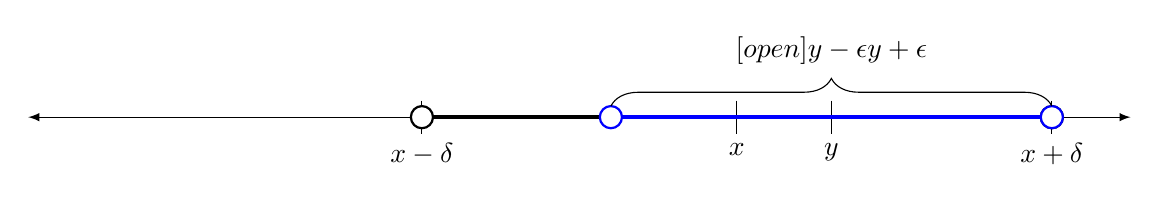
\begin{tikzpicture}[scale=2.]
          \draw[latex-latex] (-3.5,0) -- (3.5,0) ;
          \draw[shift={(1,0)},color=black] (0pt,3pt) -- (0pt,-3pt) node[below] {$x$};
          \draw[shift={(-1,0)},color=black] (0pt,3pt) -- (0pt,-3pt) node[below] {$x-\delta$};
          \draw[shift={(3,0)},color=black] (0pt,3pt) -- (0pt,-3pt) node[below] {$x+\delta$};
          \draw[very thick] (-1,0) -- (3,0);
          \path [draw=black, fill=white, thick] (-1,0) circle (2pt);
          \path [draw=black, fill=white, thick] (3,0) circle (2pt);

          \draw[shift={(1.6,0)},color=black] (0pt,3pt) -- (0pt,-3pt) node[below] {$y$};
          \draw[very thick,color=blue] (0.2,0) -- (3,0);
          \path [draw=blue, fill=white, thick] (0.2,0) circle (2pt);
          \path [draw=blue, fill=white, thick] (3,0) circle (2pt);
          
          \draw [decorate,decoration={brace,amplitude=10pt},yshift=2pt] (0.2,0) -- (3,0) node [black,midway,yshift=20pt] {$\interval[open]{y-\epsilon}{y+\epsilon}$};
        \end{tikzpicture}
      \end{figure}
      $\interval[open]{y-\epsilon}{y+\epsilon}$ is dan een deel van $\interval[open]{x-\delta}{x+\delta}$ en van $A$ bijgevolg zit $y$ in $V$.
      $V$ is dus een open deelverzameling van $A$ en daarom een deel van $\mathring{A}$.
    \item Elke open deelverzameling $W$ van $A$ is een deel van $V$: $V$ is dus het grootst.
      Als $W$ leeg is, is dit evident.
      Als $W$ niet leeg is, bestaat er een $x\in W$.
      Omdat $W$ open is bestaat er dan een $\delta\in \mathbb{R}_{0}^{+}$ zodat $\interval[open]{x-\delta}{x+\delta}$ een deel is van $W$ en dus van $A$.
      Dit betekent dat $x$ tot $V$ behoort.
      $W$ is een willekeurige open deelverzameling van $A$, dus ook $\mathring{A}$ is een deel van $V$.
    \end{itemize}
    We concluderen dat $\mathring{A}$ inderdaad gelijk is aan $V$.
  \end{proof}
\end{pr}

\begin{pr}
  Zij $A$ een deelverzameling van $\mathbb{R}$, dan ziet $\bar{A}$ er als volgt uit:
  \[ \bar{A} = \{ x\in \mathbb{R} \mid \forall \delta \in \mathbb{R}_{0}^{+}:\ \interval[open]{x-\delta}{ x+\delta} \cap A \neq \emptyset \} \]

  \begin{proof}
    Noem het rechterlid $F$.
    \begin{itemize}
    \item $F$ is een gesloten oververzameling van $A$.\\
      $A$ is duidelijk een deelverzameling van $F$.
      We beweren dus nog dat $F$ gesloten is, of dus dat $F^{c}$ open is.
      Als $F^{c}$ leeg is, is $F$ zeker gesloten.\stref{st:r-open-en-gesloten}
      Als $F^{c}$ niet leeg is, bestaat er een $\delta$ zodat $\interval[open]{x-\delta}{x+\delta} \cap A$ leeg is.
      $\interval[open]{x-\delta}{x+\delta}$ zit dus in $A^{c}$ en bijgevolg in $F^{c}$.\waarom
      $F$ is dus een gesloten oververzameling van $A$: $\bar{A} \subseteq F$.
    \item Elke gesloten oververzameling $G$ van $A$ is een oververzameling van $F$.\\
      $G^{c}$ is dan een deel van $A^{c}$.
      We beweren dat $G^{c}$ een deel is van $F^{c}$.
      Als $G^{c}$ leeg is, is dit triviaal waar.
      Als $G^{c}$ niet leeg is, dan bestaat er een $x\in G^{c}$.
      Omdat $G$ gesloten is, is $G^{c}$ open en dus kunnen we een $\delta \in \mathbb{R}_{0}^{+}$ vinden zodat $\interval[open]{x-\delta}{x+\delta}$ een deel is van $G^{c}$ en dus van $A^{c}$.
      De doorsnede van $\interval[open]{x-\delta}{x+\delta}$ en $A$ is dus leeg en daarom is $x$ een element van $F^{c}$.
      We vinden $G^{c}\subseteq F^{c}$ en daarom $F \subseteq G$.
      Omdat dit geldt voor elke gesloten oververzameling $G$, geldt het ook voor $F$: $F \subseteq \bar{A}$.
    \end{itemize}
    We concluderen dat $\bar{A}$ inderdaad gelijk is aan $F$.
  \end{proof}
\end{pr}

\begin{de}
  We noemen een punt $x$ van niet-lege deelverzameling $A$ van $\mathbb{R}$ een \term{inwendig punt} van $A$ als het tot $\mathring{A}$ behoort.
  \[ \exists \delta \in \mathbb{R}_{0}^{+}: \interval[open]{x-\delta}{x+\delta} \subseteq A \]
\end{de}

\begin{de}
  We noemen een punt $x$ van niet-lege deelverzameling $A$ van $\mathbb{R}$ een \term{adherent punt} aan $A$ als het tot $\bar{A}$ behoort.
  \[ \forall \delta \in \mathbb{R}_{0}^{+}:\ \interval[open]{x-\delta}{x+\delta} \cap A \neq \emptyset \]
\end{de}

\begin{pr}
  Zij $A$ een deel van $\mathbb{R}$ en $x\in \mathbb{R}$, dan behoort $x$ tot $\bar{A}$ als en slechts als er een rij $(x_{n})_{n}$ in $A$ bestaat met $x$ als limiet.

  \begin{proof}
    Bewijs van een equivalentie:
    \begin{itemize}
    \item $\Rightarrow$\\
      Zij $x$ een adherent punt.
      Als $x$ tot $A$ behoort heeft de constante rij $(x)_{n}$ $x$ als limiet.
      Stel daarom dat $x$ tot $\bar{A}\setminus A$ behoort.
      Voor elke $n\in \mathbb{N}$ is $\interval[open]{x-\frac{1}{n}}{x+\frac{1}{n}} \cap A$ niet leeg (omdat $x$ een adherent punt is).
      Kies dus voor elke $n$ een $x_{n} \in \interval[open]{x-\frac{1}{n}}{x+\frac{1}{n}}$ om een rij $(x_{n})_{n}$ te bekomen met $x$ als limiet.
    \item $\Leftarrow$\\
      Zij $(x_{n})_{n}$ een rij met limiet $x\in A$. We bewijzen dat $x$ een adherent punt is aan $A$.
      Kies daartoe een willekeurige $\delta \in \mathbb{R}_{0}^{+}$.
      Er bestaat dan een $n_{0}\in \mathbb{N}$ zodat voor alle volgende $n\in\mathbb{N}$ $x_{n}$ in $\interval[open]{x-\delta}{x+\delta}$ zit.
      Omdat $(x_{n})_{n}$ een rij is in $A$ behoort $x_{n}$ ook tot $A$.
      De doorsnede van $A$ en $\interval[open]{x-\delta}{x+\delta}$ bevat dus al zeker $x_{n}$ en is bijgevolg niet leeg.
    \end{itemize}
  \end{proof}
  \feed
\end{pr}

\subsection{Randpunten, ge\"isoleerde punten en ophopingspunten.}
\label{sec:randp-geis-punt}

\begin{de}
  De \term{rand} $\partial A$ van een deelverzameling $A$ van $\mathbb{R}$ definieren we als volgt:
  \[ \partial A = \bar{A} \setminus \mathring{A} \]
\end{de}

\begin{de}
  Een \term{randpunt} van een deelverzameling $A$ van $\mathbb{R}$ is een element van de rand $\partial A$ van $A$.
\end{de}

\begin{st}
  Een punt $x\in \mathbb{R}$ is een randpunt van een deelverzameling $A$ van $\mathbb{R}$ als en slechts het volgende geldt:
  \[ \forall \delta \in \mathbb{R}_{0}^{+}:\ ]x-\delta,x+\delta[ \cap A \neq \emptyset\ \wedge\  ]x-\delta,x+\delta[ \cap A^{c} \neq \emptyset \]

  \begin{proof}
    Een randpunt $x$ van een deelverzameling $A$ van $\mathbb{R}$ is een adherent punt dat geen inwendig punt is.
    Het eerste deel van de conjunctie is waar omdat $A$ een adherent punt is.
    Omdat $A$ geen inwendig punt is geldt het volgende:
    \[ \forall \delta \in \mathbb{R}_{0}^{+}: \interval[open]{x-\delta}{x+\delta} \not\subseteq A \]
    Dit betekent dat er voor elke $\delta \in \mathbb{R}_{0}^{+}$ een element in $\interval[open]{x-\delta}{x+\delta}$ niet tot $A$ behoort (maar dus wel tot $A^{c}$).
    De doorsnede van $\interval[open]{x-\delta}{x+\delta}$ en $A^{c}$ is dus niet leeg.
  \end{proof}
  \feed
\end{st}

\begin{de}
  Zij $A$ een niet-lege deelverzameling van $\mathbb{R}$, dan noemen we een punt $x\in A$ een \term{ge\"isoleerd punt} van $A$ als het volgende geldt:
  \[ \exists \delta \in \mathbb{R}_{0}^{+}:\ \interval[open]{x-\delta}{x+\delta} \cap A = \{ x \} \]
\end{de}

\begin{de}
  Zij $A$ een niet-lege deelverzameling van $\mathbb{R}$, dan noemen we een punt $x\in A$ een \term{ophopingspunt} of \term{accumulatiepunt} van $A$ als het volgende geldt:
  \[ \forall \delta \in \mathbb{R}_{0}^{+}:\ \interval[open]{x-\delta}{x+\delta} \cap (A \setminus \{x\}) \neq \emptyset \]
\end{de}

\begin{opm}
  Een punt $x$ in een niet-lege deelverzameling $A$ van $\mathbb{R}$, dan is $x$ ofwel een ge\"isoleerd punt, ofwel een ophopingspunt.
\end{opm}

\begin{pr}
  \label{pr:equivalenties-ophopingspunt}
  Zij $A$ een niet een niet-lege deelverzameling van $\mathbb{R}$, dan zijn volgende uitspraken equivalent.
  \begin{enumerate}
  \item $x$ is een ophopingspunt van $A$.
  \item Voor alle $\delta > 0$ bevat $\interval[open]{x-\delta}{x+\delta} \cap A$ oneindig veel punten.
  \item Er bestaat een rij $(x_{n})_{n}$ in $A\setminus \{x\}$ die naar $x$ convergeert.  
  \end{enumerate}

  \begin{proof}
    Equivalentie vanuit circulaire implicaties
    \begin{itemize}
    \item $(1) \Rightarrow (3)$\\
      Uit de definite van een ophopingspunt volgt dat voor elke $n\in \mathbb{N}$ de verzameling $\interval[open]{x-\frac{1}{n}}{x+\frac{1}{n}}\cap (A \setminus \{x\})$ niet leeg is.
      Voor elke $n$ kunnen we er dus een $x_{n}$ in kiezen om een rij $(x_{n})_{n}$ te construeren die $x$ als limiet heeft.
    \item $(3) \Rightarrow (2)$\\
      Stel dat er een $\delta \in \mathbb{R}_{0}^{+}$ bestaat zodat $\interval[open]{x-\delta}{x+\delta} \cap A$ eindig is, dan bestaat er in die verzameling een punt dat het dichtst bij $x$ ligt.
      Noem dit punt $y$ en noem de afstand tot $x$ $\epsilon = |y-x|$.
      Dit houdt in dat de verzameling $\interval[open]{x-\epsilon}{x+\epsilon} \cap A$ leeg is.
      Omdat de rij $(x_{n})_{n}$ in $A\setminus \{x\}$ naar $x$ convergeert, moet er echter een $n_{0}\in\mathbb{N}$ bestaan zodat alle voor volgende $n\in \mathbb{N}$ $x_{n}$ in $\interval[open]{x-\epsilon}{x+\epsilon}$ moet liggen.
      Omdat de rij in  $A\setminus \{x\}$ ligt moeten die $x_{n}$ dus ook in $\interval[open]{x-\epsilon}{x+\epsilon} \cap A$ liggen, maar dit is in tegenspraak met het feit dat deze verzameling leeg is.
    \item $(2) \Rightarrow (1)$\\
      Voor elke $\delta \in \mathbb{R}_{0}^{+}$ bevat $\interval[open]{x-\delta}{x+\delta} \cap A$ oneindig veel punten.
      $\interval[open]{x-\delta}{x+\delta} \cap (A \setminus \{x\})$ bevat dan nog steeds oneindig veel punten en is dus niet leeg.
    \end{itemize}
  \end{proof}
  \feed
\end{pr}

\begin{st}
  De \term{stelling van Bolzano-Weierstra\ss} (ophopingspuntversie).
  Elk oneindig begrensd deel van $\mathbb{R}$ heeft minstens \'e\'en ophopingspunt.

  \begin{proof}
    Zij $A$ een oneindige begrensde deelverzameling van $\mathbb{R}$.
    Kies nu een aftelbaar oneindige deelverzameling $B$ van $A$ en nummer de elementen van $B$ om een rij $(x_{n})_{n}$ te bekomen.
    Merk op dat die rij in $A$ ligt en dus begrensd is.
    Er bestaat dus een convergente deelrij $(x_{n_{k}})_{k}$\stref{st:bolzano-rijen}.
    Noem de limiet van deze deelrij $x$.
    We beweren dat $x$ een ophopingspunt is van $A$.
    Kies nu een $\delta \in \mathbb{R}_{0}^{+}$.
    Er bestaat dan een $k_{0}\in\mathbb{N}$ zodat voor alle volgende $k\in \mathbb{N}$ $x_{n_{k}}$ dichter dan $\delta$ bij $x$ ligt.
    Het interval $\interval[open]{x-\delta}{x+\delta}$ bevat dan oneindig veel punten (tenminste alle $x_{n_{k}}$ met $k>k_{0}$).
    Bijgevolg is $x$ een ophopingspunt van $A$.\prref{pr:equivalenties-ophopingspunt}
  \end{proof}
\end{st}

\subsection{Relatieve topologie}
\label{sec:relatieve-topologie}

\begin{de}
  We noemen een deelverzameling $A$ van $X\subseteq \mathbb{R}$ \term{relatief open} in $X$ als het volgende geldt:
  \[ \forall x\in A:\ \exists \delta \in \mathbb{R}_{0}^{+}:\ \forall y\in X:\ |y-x| < \delta \Rightarrow y \in A \]
\end{de}

\begin{st}
  Een  deelverzameling $A$ van $X\subseteq \mathbb{R}$  is relatief open in $X$ als en slechts als het volgende geldt:
  \[ \forall x\in A:\ \exists \delta\in \mathbb{R}_{0}^{+}:\ \interval[open]{x-\delta}{x+\delta} \cap X \subseteq A \]
  \extra{bewijs}
\end{st}

\begin{de}
  We noemen een deelverzameling $A$ van $X\subseteq \mathbb{R}$ \term{relatief gesloten} in $X$ als het relatief complement $X\setminus B$ van $B$ relatief open is in $X$.
\end{de}

\begin{pr}
  Zij $X$ een niet-leeg deel van $\mathbb{R}$ en $A \subseteq X$.
  $A$ is relatief open in $X$ als en slechts als er een open $V\subseteq \mathbb{R}$ bestaat zodat $A=V \cap X$ geldt.

  \begin{proof}
    Bewijs van een equivalentie\\
    \begin{itemize}
    \item $\Rightarrow$\\
      Als $A$ leeg is kunnen we voor $V$ $\emptyset$ nemen.
      Als $A$ niet leeg is, dan bestaat er een $x\in A$.
      We kunnen dan een $\delta_{x}$ kiezen zodat $\interval[open]{x-\delta}{x+\delta} \cap X$ een deel is van $A$.
      Benoem nu $V$ als volgt:
      \[ \bigcup_{x\in A}\interval[open]{x-\delta_{x}}{x+\delta_{x}} \]
      $V$ is dan een open deel van $\mathbb{R}$ want het is een unie van open verzamelingen.\prref{pr:unie-open-verzamelingen-open}
      Bovendien is $A$ per constructie de doorsnede van $V$ en $X$.
    \item $\Leftarrow$\\
      Zij $X$ een niet-leeg deel van $\mathbb{R}$ en $V$ een open deel van $\mathbb{R}$.
      We bewijzen dan dat $A$ relatief open is in $V\cap X$.
      Kies daartoe een $x\in A$. Er bestaat dan een $\delta\in \mathbb{R}_{0}^{+}$ zodat $\interval[open]{x-\delta}{x+\delta}$ in $V$ zit.
      De doorsnede van dit interval en $X$ is dan een deel van $V \cap X$.
      $V\cap X$ is dus een open deel van $X$.
    \end{itemize}
  \end{proof}
\end{pr}

\begin{pr}
  Zij $X$ een niet-leeg deel van $\mathbb{R}$ en $A \subseteq X$.
  $A$ is relatief gesloten in $X$ als en slechs als er een gesloten $F \subseteq \mathbb{R}$ bestaat zodat $A=F \cap X$ geldt.
  \TODO{oefening}
\end{pr}

\section{De complexe getallen}
\label{sec:de-complexe-getallen}

\subsection{Het veld van de complexe getallen}
\label{sec:het-veld-van}


\begin{de}
  De verzameling $\mathbb{C}$ van \term{complexe getallen} defini\"eren we als volgt, samen met de optelling $(+)$ en vermenigvuldiging $(\cdot)$.
  \[ \mathbb{C} = \mathbb{R}^{2} = \{ (a,b) \mid a,b\in \mathbb{R} \} \]
  \[ (+):\ \mathbb{C}^{2} \rightarrow \mathbb{C}:\ (a,b) + (c,d) = (a+c,b+d) \]
  \[ (\cdot):\ \mathbb{C}^{2} \rightarrow \mathbb{C}:\ (a,b) \cdot (c,d) = (ac-bd, ad+bc) \]
\end{de}

\begin{st}
  $\mathbb{C},+,\cdot$ is een veld.
  \extra{bewijs p 81}
\end{st}

\begin{pr}
  We kunnen $\mathbb{R}$ inbedden in $\mathbb{C}$ met de volgende injectieve afbeelding:
  \[ \phi:\ \mathbb{R} \rightarrow \mathbb{C}:\ a \mapsto (a,0) \]
  Deze afbeelding is bovendien een ringmorfisme:
  \[ \forall a,b \in \mathbb{R}:\ \phi(a+b) = \phi(a) + \phi(b) \]
  \[ \forall a,b \in \mathbb{R}:\ \phi(ab) = \phi(a)\phi(b) \] 
  \extra{bewijs: oefening}
\end{pr}

\begin{opm}
  Onder deze injectie beschouwen we $\mathbb{R}$ als een deelveld van $\mathbb{C}$.
\end{opm}

\begin{de}
  We noteren een element $(a,b)$ van $\mathbb{C}$ vaak als $a+bi$.
  We noemen dit de \term{carthesiaanse vorm van een complex getal}.
\end{de}

\begin{opm}
  Deze notatie komt van pas om rekenregels binnen $\mathbb{C}$ eenvoudig te houden als we $i^{2}=1$ als regel in het achterhoofd houden. 
  \extra{bewijs!}
\end{opm}

\begin{de}
  We noemen in een element $a+bi$ van $\mathbb{C}$ $a$ het \term{re\"eel} deel en $b$ het \term{imaginair} deel.
  We voeren daarom twee afbeeldingen in:
  \[ Re:\ \mathbb{C} \rightarrow \mathbb{R}:\ (a+bi) \mapsto a \]
  \[ Im:\ \mathbb{C} \rightarrow \mathbb{R}:\ (a+bi) \mapsto b \]
\end{de}

\begin{st}
  De \term{hoofdstelling van de algebra}\\
  $\mathbb{C}$ is algebra\"isch gesloten: Een $n$-de graadsveelterm over $\mathbb{C}$ heeft precies $n$ wortels in $\mathbb{C}$.
  \zb
\end{st}

\begin{pr}
  Er bestaat geen orde op $\mathbb{C}$ die van $\mathbb{C},+,\cdot$ een totaal geordend veld maakt.

  \begin{proof}
    Bewijs uit het ongerijmde: stel dat er wel zo'n orde $\le$ bestaat.
    Dan moet $i$ ofwel groter dan $0$ zijn, ofwel kleiner dan nul.
    In beide gevallen volgt $-1 > 0$ of $1 < 0$,\prref{pr:geordend-veld-ongelijkheid-vermenigvuldiging} wat niet mogelijk is in een geordende veld.\prref{pr:nul-kleiner-dan-een}
  \end{proof}
\end{pr}

\begin{de}
  Het \term{complex toegevoegde} $\overline{a+bi}$ van een complex getal $a+bi$ definieren we als volgt:
  \[ \overline{a+bi} = a-bi \]
  \[ \overline{\, \cdot\ }:\ \mathbb{C} \rightarrow \mathbb{C}:\ a+bi \mapsto \overline{a+bi} = a-bi \]
\end{de}

\begin{de}
  De \term{modulus} $|a+bi|$ van een complex getal $a+bi$ definieren we als volgt:
  \[ |a+bi| = \sqrt{a^{2}+b^{2}} \]
  \[ |\cdot|:\ \mathbb{C} \rightarrow \mathbb{R}:\ a+bi \mapsto |a+bi| = \sqrt{a^{2}+b^{2}} \]
\end{de}

\begin{ei}
  De modulus van een complex getal is de tegenhanger van de absolute waarde van een re\"eel getal.
  \[ \forall a \in \mathbb{R}:\ |a| = |\phi(a)| \]
  \begin{proof}
    $\forall a\in \mathbb{R}:\ |\phi(a)| = |a+0i| = \sqrt{a^{2} + 0^{2}} = |a|$
  \end{proof}
\end{ei}

\begin{pr}
  \[ \forall z\in \mathbb{C}:\ \bar{\bar{z}} = z \]

  \begin{proof}
    $\forall a+bi\in \mathbb{C}:\ \bar{\bar{a+bi}} = \bar{a-bi} = a-(-bi) = a+bi$
  \end{proof}
\end{pr}

\begin{pr}
  \[ \forall z_{1},z_{2}\in \mathbb{C}:\ \overline{z_{1}+z_{2}} = \overline{z_{1}} + \overline{z_{2}} \]

  \begin{proof}
    $\forall a+bi,c+di \in \mathbb{C}:\ \overline{a+bi + c+di} = \overline{(a+c)+(b+d)i} =(a+c)-(b+d)i = a+c-bi-di = (a-bi) + (c-di)$
  \end{proof}
\end{pr}

\begin{pr}
  \[ \forall z_{1},z_{2}\in \mathbb{C}:\ \overline{z_{1}z_{2}} = \bar{z}_{1}  \bar{z}_{2} \]

  \begin{proof}
    $\forall a+bi,c+di \in \mathbb{C}:\ \overline{a+bi \cdot c+di} = \overline{ac-bd + (ad+bc)i} = ac-bd - adi - bci = ac-(-b)(-d) + (a(-d)+(-b)c)i = \overline{a+bi} \cdot \overline{c+di} $
  \end{proof}
\end{pr}

\begin{pr}
  \[ \forall z\in \mathbb{C}:\ Re(z) = \frac{z+\bar{z}}{2} \]

  \begin{proof}
    $\forall a+bi\in \mathbb{C}:\ \frac{(a+bi)+\overline{a+bi}}{2} = \frac{(a+bi)+(a-bi)}{2} = \frac{2a}{2} = a = Re(a+bi)$
  \end{proof}
\end{pr}

\begin{pr}
  \[ \forall z\in \mathbb{C}:\ Im(z) = \frac{z-\bar{z}}{2i} \]

  \begin{proof}
    $\forall a+bi\in \mathbb{C}:\ \frac{(a+bi)-\overline{a+bi}}{2i} = \frac{(a+bi)-(a-bi)}{2i} = \frac{(a+bi-a+bi)}{2i} = \frac{2bi}{2i} = b = Im(a+bi) $
  \end{proof}
\end{pr}

\begin{pr}
  \[ \forall z\in \mathbb{C}:\ |\bar{z}| = |z| \]

  \begin{proof}
    $\forall a+bi\in \mathbb{C}:\ |\bar{a+bi}| = |a-bi| = \sqrt{a^{2}+(-b)^{2}} = \sqrt{a^{2}+b^{2}} = |a+bi|$
  \end{proof}
\end{pr}

\begin{pr}
  \label{pr:reel-deel-kleine}
  \[ \forall z\in \mathbb{C}:\ |Re(z)| \le |z| \]

  \begin{proof}
    $\forall a+bi\in \mathbb{C}:\  |Re(a+bi)| = |a| \le \sqrt{a^{2}+b^{2}} = |a+bi|$ 
  \end{proof}
\end{pr}

\begin{pr}
  \label{pr:imaginair-deel-kleiner}
  \[ \forall z\in \mathbb{C}:\ |Im(z)| \le |z|\]

  \begin{proof}
    $\forall a+bi\in \mathbb{C}:\  |Im(a+bi)| = |b| \le \sqrt{a^{2}+b^{2}} = |a+bi|$ 
  \end{proof}
\end{pr}

\begin{pr}
  \[ \forall z\in \mathbb{C}:\ \bar{z}z\in \mathbb{R} \]

  \begin{proof}
    $\forall a+bi\in \mathbb{C}:\  \overline{a+bi}\cdot(a+bi) = (a-bi)(a+bi) = a^{2} + (-bi)a + a(bi) + (-bi)(bi) = a^{2} + b^{2} \in \mathbb{R}$
  \end{proof}
\end{pr}

\begin{pr}
  \[ \forall z\in \mathbb{C}:\ |z| = \sqrt{\bar{z}z} \]

  \begin{proof}
    $\forall a+bi\in \mathbb{C}:\ \sqrt{\overline{a+bi}\cdot(a+bi)} = \sqrt{a^{2}+b^{2}} = |a+bi|$
  \end{proof}
\end{pr}

\begin{pr}
  \[ \forall z\in \mathbb{C}:\ \forall z \in \mathbb{C}_{0}: \frac{1}{z} = \frac{\bar{z}}{|z|^{2}} \]

  \begin{proof}
    $\forall a+bi\in \mathbb{C}:\ \frac{\overline{a+bi}}{|a+bi|^{2}} = \frac{a-bi}{\left(\sqrt{a^{2}+b^{2}}\right)^{2}} = \frac{a-bi}{a^{2}+b^{2}}= \frac{(a-bi)(a+bi)}{(a^{2}+b^{2})(a+bi)} = \frac{a^{2}+b^{2}}{(a^{2}+b^{2})(a+bi)} = \frac{1}{a+bi}$
  \end{proof}
\end{pr}

\begin{pr}
  \[ \forall z_{1},z_{2}\in \mathbb{C}:\ |z_{1}z_{2}| = |z_{1}||z_{2}| \]

  \begin{proof}
    \[
    \forall a+bi,c+di \in \mathbb{C}:\
    \begin{array}{rll}
      |(a+bi)(c+di)| &= |ac-bd + (ad+bc)i|\\
      &= \sqrt{(ac-bd)^{2} + (ad+bc)^{2}}\\
      &= \sqrt{a^{2}c^{2} +b^{2}d^{2}-2abcd + a^{2}d^{2} + b^{2}c^{2} +2abcd}\\
      &= \sqrt{a^{2}c^{2} +b^{2}d^{2} + a^{2}d^{2} + b^{2}c^{2}}\\
      &= \sqrt{a^{2}+b^{2}}\sqrt{c^{2}+d^{2}}
    \end{array}
    \]
  \end{proof}
\end{pr}

\begin{pr}
  \[ \forall z_{1},z_{2}\in \mathbb{C}:\ |z_{1}+z_{2}| \le |z_{1}|+|z_{2}| \]

  \begin{proof}
    \[
    \forall a+bi,c+di \in \mathbb{C}:\
    \begin{array}{rll}
      |(a+bi)+(c+di)|^{2} &= |(a+c)+(b+d)i|^{2}\\
      &= (a+c)^{2}+ (b+d)^{2}\\
      &= a^{2}+c^{2} + b^{2}+d^{2}+2(ac + bd)\\
      &= a^{2}+c^{2} + b^{2}+d^{2}+2Re((a-bi)(c+di))\\
      &\le a^{2}+b^{2} + c^{2}+d^{2} + 2|(a-bi)(c+di)|\\
      &= a^{2}+b^{2} + c^{2}+d^{2} + 2\sqrt{a^{2}c^{2} + a^{2}d^{2} +b^{2}c^{2}+ b^{2}d^{2}}\\
      &= a^{2}+b^{2} + c^{2}+d^{2} + 2\sqrt{(a^{2}+b^{2})(c^{2}+d^{2})}\\
      &= |a+bi|^{2} + |c+di|^{2} + 2|a+bi||c+di|\\
      &= \left(|a+bi|+|c+di|\right)^{2}\\
    \end{array}
    \]
  \end{proof}
\end{pr}

\begin{pr}
  \label{pr:tweede-driehoeksongelijkheid-C}
  \[ \forall x,y,z\in \mathbb{C}:\ |x-z| \le |x-y| + |y-z| \]

  \begin{proof}
    Gebruik de driehoeksongelijkheid op $|(x-y)+(y-z)| \le |x-y| + |y-z|$
  \end{proof}
\end{pr}

\begin{pr}
  \[ \forall z_{1},z_{2}\in \mathbb{C}:\ ||z_{1}|-|z_{2}|| \le |z_{1}-z_{2}| \]

  \begin{proof}
    \[ |x| + |y-x| \ge |x+y-x| = |y| \]
    \[ |y| + |x-y| \ge |y+x-y| = |x| \]
    Verplaats in beide ongelijkheden de linker term naar de rechterkant:
    \[ |y-x| \ge |y| - |x| \]
    \[ |x-y| \ge |x| - |y| \]
    $|y-x|$ is gelijk aan $|x-y|$. Hieruit, samen met $t \ge a \wedge t \ge -a \Rightarrow t \ge |a|$ volgt de stelling:
    \[ |x-y| \ge \left||x|-|y|\right| \]
    \extra{gebruikte stelling afsplitsen}
  \end{proof}
\end{pr}

\begin{de}
  Zij $z = a+bi$ de carthesiaanse co\"ordinaten van een complex getal, dan definieren we de \term{poolcoordinaten} van dat getal als $(r,\theta)$:
  \[ a = r \cos \theta \quad\text{ en }\quad b = r\sin \theta \]
  \[ z = r(\cos \theta + i \sin \theta)  \]
\end{de}

\begin{st}
  \label{st:vermenigvuldiging-poolcoordinaten}
  \[
  \forall z_{1},z_{2} \in \mathbb{C}:\ 
  r_{1}(\cos \theta_{1} + i \sin \theta_{1}) \cdot r_{2}(\cos \theta_{2} + i \sin \theta_{2})
  = r_{1}r_{2}\left(\cos(\theta_{1}+\theta_{2}) + i\sin(\theta_{1}+\theta_{2})\right)
  \]
  
  \[ 
  \begin{array}{l}
    \forall z_{1},z_{2} \in \mathbb{C}:\\
    r_{1}(\cos \theta_{1} + i \sin \theta_{1}) \cdot r_{2}(\cos \theta_{2} + i \sin \theta_{2})\\
    = r_{1}r_{2} (\cos \theta_{1} + i \sin \theta_{1})(\cos \theta_{2} + i \sin \theta_{2})\\
    = r_{1}r_{2} \left( \left(\cos \theta_{1}\cos \theta_{2} -\sin \theta_{1}\sin \theta_{2}\right)+ i\left( \sin \theta_{1}\cos \theta_{2} + \cos \theta_{1}\sin \theta_{2}\right)  \right)\\
    = r_{1}r_{2}\left(\cos(\theta_{1}+\theta_{2}) + i\sin(\theta_{1}+\theta_{2})\right)\\
  \end{array}
  \]
\end{st}

\begin{st}
  De \term{formule van de Moivre}\\
  \[ \forall z = r(\cos \theta + i \sin \theta) \in \mathbb{C}, n\in \mathbb{Z}:\ (r(\cos \theta + i \sin \theta))^{n} = r^{n}(\cos n\theta + i \sin n\theta)\]

  \begin{proof}
    Gevalsonderscheid
    \begin{itemize}
    \item Voor alle $n\in \mathbb{N}$ volgt dit meteen uit stelling
      \ref{st:vermenigvuldiging-poolcoordinaten}.
    \item Voor $n=-1$:
      \[
      \begin{array}{rl}
        (r(\cos \theta + i \sin \theta))^{-1}
        &= \frac{1}{r(\cos \theta + i \sin \theta)}\\
        &= \frac{\cos \theta - i \sin \theta}{r(\cos \theta + i \sin \theta)(\cos \theta - i \sin \theta)}\\
        &= \frac{\cos(\theta) - i\sin(\theta)}{r}\\
        &= r^{-1}\cos(-\theta) + i\sin(-\theta)\\
      \end{array}
      \]
    \item Voor $-n\in \mathbb{Z}^{-}$ komt een $-n$-de macht met een $n$-de macht en een $-1$-e macht na elkaar.
    \end{itemize}
  \end{proof}
\end{st}


\begin{de}
  We noemen $z\in \mathbb{C}$ een $n$-de \term{eenheidswortel} als het volgende geldt:
  \[ z^{n} = 1 \]
  Merk op dat er voor graad $n$ precies $n$ eenheidswortel zijn:
  \[ z = \cos\left(\frac{2k\pi}{n}\right) + i \sin \left( \frac{2k\pi}{n} \right) \]
  \extra{afsplitsen in stelling?}
\end{de}


\subsection{Rijen in $\mathbb{C}$}
\label{sec:rijen-mathbbc}

\begin{de}
  We zeggen dat een rij $(x_{n})_{n}$ in $\mathbb{C}$ \term{convergeert} naar een element $c\in \mathbb{C}$ als en slechts als het volgende geldt:
  \[ \forall \epsilon \in \mathbb{R}_{0}^{+}:\ \exists n_{0}\in \mathbb{N}:\ \forall n\in \mathbb{N}:\ n \ge n_{0} \Rightarrow |z_{n}-c| < \epsilon \]
  We noemen $c$ de \term{limiet} van de rij $(x_{n})_{n}$.
  \[ \lim_{n\rightarrow +\infty}z_{n} = c \]
\end{de}

\begin{de}
  Een rij die convergeert noemen we een \term{convergente} rij.
\end{de}

\begin{pr}
  \label{pr:complexe-limiet-splitsen}
  Zij $(z_{n})_{n}$ een rij in $\mathbb{C}$.
  Noem $x_{n} = Re(z_{n})$ en $y_{n} = Im(z_{n})$.
  Noem bovendien $a=Re(c)$ en $b=Im(c)$.
  $(z_{n})_{n}$ convergeert naar $c$ als en slechts als $(x_{n})_{n}$ naar $a$ en $(y_{n})_{n}$ naar $b$ convergeert.

  \begin{proof}
    Merk eerst op dat de volgende ongelijkheid geldt door $x_{n}$, $a$, $y_{n}$ en $b$ te beschouwen als complexe getallen.\prref{pr:tweede-driehoeksongelijkheid-C}
    \[ |z_{n}-c| \le |x_{n}-a| + |y_{n}-b| \]
    Er gelden ook de volgende ongelijkheden.\prref{pr:reel-deel-kleine}\prref{pr:imaginair-deel-kleiner}
    \[ |x_{n}-a| \le |z_{n}-c| \]
    \[ |y_{n}-b| \le |z_{n}-c| \]
    \begin{itemize}
    \item $\Rightarrow$
      Kies een wilekeurige $\delta \in \mathbb{R}_{0}^{+}$.
      Vanwege de tweede en derde ongelijkheid worden $|x_{n}-a|$ en $|y_{n}-b|$ kleiner dan $\delta$ vanaf een bepaalde $n\in \mathbb{N}$ omdat $z_{n}$ convergeert naar $c$.
    \item $\Leftarrow$
      Kies een willekeurige $\delta \in \mathbb{R}_{0}^{+}$.
      Er bestaan dan een $n_{x},n_{y}\in \mathbb{N}$ zodat $|x_{n}-a|$ en $|y_{n}-b|$ kleiner worden dan $\frac{\delta}{2}$ voor $n$ groter dan $n_{x}$, respectievelijk $n_{y}$.
      Vanaf $\max\{n_{x},n_{y}\}$ geldt dan het volgende vanwege de eerste ongelijkheid:
      \[ |z_{n}-c| \le |x_{n}-a| + |y_{n}-b| < \frac{\delta}{2}+\frac{\delta}{2} = \delta \]
    \end{itemize}
  \end{proof}
  \extra{dit kan mooier?}
\end{pr}

\begin{st}
  \label{st:bolzano-complexe-rijen}
  De \term{stelling van Bolzano-Weierstra\ss} voor complexe rijen\\
  Elke begrensde rij in $\mathbb{C}$ heeft een convergente deelrij.

  \begin{proof}
    Zij $(z_{n})_{n}$ een begrensde rij in $\mathbb{C}$
    Noem $x_{n} = Re(z_{n})$ en $y_{n} = Im(z_{n})$.
    De rijen $(x_{n})_{n}$ en $(y_{n})_{n}$ zijn dan begrensde rijen in $\mathbb{R}$\prref{pr:tweede-driehoeksongelijkheid-C}
    We kunnen dus twee convergente deelrijen $(x_{n_{k}})_{k}$ en $(y_{n_{k}})_{k}$ vinden.\stref{st:bolzano-rijen}
    Noem de limieten respectievelijk $a$ en $b$.
    De deelrij $(z_{n_{k}})_{k}$ van $(z_{n})_{n}$ convergeert dan naar $a+bi$.\prref{pr:complexe-limiet-splitsen}
  \end{proof}
\end{st}

\begin{de}
  We noemen een rij $(z_{n})_{n}$ in $\mathbb{C}$ een \term{Cauchyrij} als en slechts als het volgende geldt:
  \[ \forall \epsilon \in \mathbb{R}_{0}^{+}:\ \exists n_{0}\in \mathbb{N}:\ \forall n,m\in \mathbb{N}_{0}: n,m\ge n_{0} \Rightarrow |z_{n}-z_{m}| < \epsilon \]
\end{de}

\begin{pr}
  Zij $(z_{n})_{n}$ een rij in $\mathbb{C}$.
  Noem $x_{n} = Re(z_{n})$ en $y_{n} = Im(z_{n})$.
  $(z_{n})_{n}$ is een Cauchyrij als en slechts als $(x_{n})_{n}$ en $(y_{n})_{n}$ Cauchyrijen zijn.

  \begin{proof}
    We beginnen opnieuw met drie ongelijkheden:
    \[ |z_{n}-z_{m}| \le |x_{n}-x_{m}| + |y_{n}-y_{m}| \]
    \[ |x_{n}-x_{m}| \le |z_{n}-z_{m}| \]
    \[ |y_{n}-y_{m}| \le |z_{n}-z_{m}| \]
    \begin{itemize}
    \item $\Rightarrow$\\
      Kies een willekeurige $\delta \in \mathbb{R}_{0}^{+}$.
      Vanwege de tweede en derde ongelijkheid worden $|x_{n}-x_{m}|$ en $|y_{n}-y_{m}|$ kleiner dan $\delta$ vanaf een bepaalde $n\in \mathbb{N}$ omdat $z_{n}$ een Cauchyrij is.
    \item $\Leftarrow$\\
      Kies een willekeurige $\delta \in \mathbb{R}_{0}^{+}$.
      Er bestaan dan een $n_{x},n_{y}\in \mathbb{N}$ zodat $|x_{n}-x_{m}|$ en $|y_{n}-y_{m}|$ kleiner worden dan $\frac{\delta}{2}$ voor $n,m$ groter dan $n_{x}$, respectievelijk $n_{y}$.
      Vanaf $\max\{n_{x},n_{y}\}$ geldt dan het volgende vanwege de eerste ongelijkheid:
      \[ |z_{n}-z_{m}| \le |x_{n}-x_{m}| + |y_{n}-y_{m}| < \frac{\delta}{2}+\frac{\delta}{2} = \delta \]
    \end{itemize}
  \end{proof}
\end{pr}

\begin{st}
  Een rij $(z_{n})_{n}$ in $\mathbb{C}$ is convergent als en slechts als het een Cauchyrij is.

  \begin{proof}
    Bewijs van een equivalentie\\
    \begin{itemize}
    \item $\Rightarrow$\\
\extra{bewijs}
    \item $\Leftarrow$\\
      Noem $x_{n} = Re(z_{n})$ en $y_{n} = Im(z_{n})$.
      $(x_{n})_{n}$ en $(y_{n})_{n}$ zijn dan Cauchyrijen in $\mathbb{R}$, en convergeren dus.\prref{pr:cauchyrij-in-R-convergeert}
      Noem $a$ en $b$ de respectievelijke limieten.
      $(z_{n})_{n}$ convergeert dan naar $a+bi$.\prref{pr:complexe-limiet-splitsen}
    \end{itemize}
  \end{proof}
\end{st}

\subsection{Topologie in $\mathbb{C}$}
\label{sec:topologie-mathbbc}

\begin{de}
  We noemen een deelverzameling $A$ van $\mathbb{C}$ \term{open} als en slechts als het volgende geldt:
  \[ \forall x\in A:\ \exists \delta \in \mathbb{R}_{0}^{+}:\ \forall y\in \mathbb{C}:\ |y-x| < \delta \Rightarrow y \in A \]
\end{de}

























\end{document}
